\documentclass{article}
\usepackage[T1]{fontenc}
\usepackage[utf8]{inputenc}
\usepackage{lmodern}
\usepackage[top=25mm, bottom=25mm, left=25mm, right=25mm]{geometry}
\usepackage[english]{babel}
\usepackage{graphicx}
\usepackage{float}
\usepackage{hyperref}
\usepackage{parskip}
\usepackage{listings}
\usepackage{xcolor}
\usepackage{arev}
\usepackage{pdfpages}

\definecolor{codegreen}{rgb}{0,0.6,0}
\definecolor{codegray}{rgb}{0.5,0.5,0.5}
\definecolor{codepurple}{rgb}{0.58,0,0.82}
\definecolor{backcolour}{rgb}{0.95,0.95,0.92}

\lstdefinestyle{lststyle}{
	backgroundcolor=\color{backcolour},
	frame=single,
	framerule=0pt,
    commentstyle=\color{codegreen},
    keywordstyle=\color{magenta},
    numberstyle=\tiny\color{codegray},
    stringstyle=\color{codepurple},
    basicstyle=\ttfamily\footnotesize,
    breakatwhitespace=false,         
    breaklines=true,                 
    captionpos=b,                    
    keepspaces=true,                 
    % numbers=left,                    
    numbersep=5pt,                  
    showspaces=false,                
    showstringspaces=false,
    showtabs=false,                  
    tabsize=4
}
\lstset{style=lststyle}

\title{Afstudeerproject Systeem- en Netwerkbeheer\\
	\large Virtualizing the UCLL core network in VIRL}
\date{2020\\ February}
\author{Arne Bauters\\
	\texttt{arne.bauters@student.ucll.be}
	\and 
	Dieter Maes\\
	\texttt{dieter.maes@student.ucll.be}
	\and
	Wietse Vandeput\\
	\texttt{wietse.vandeput@student.ucll.be}
}

\begin{document}
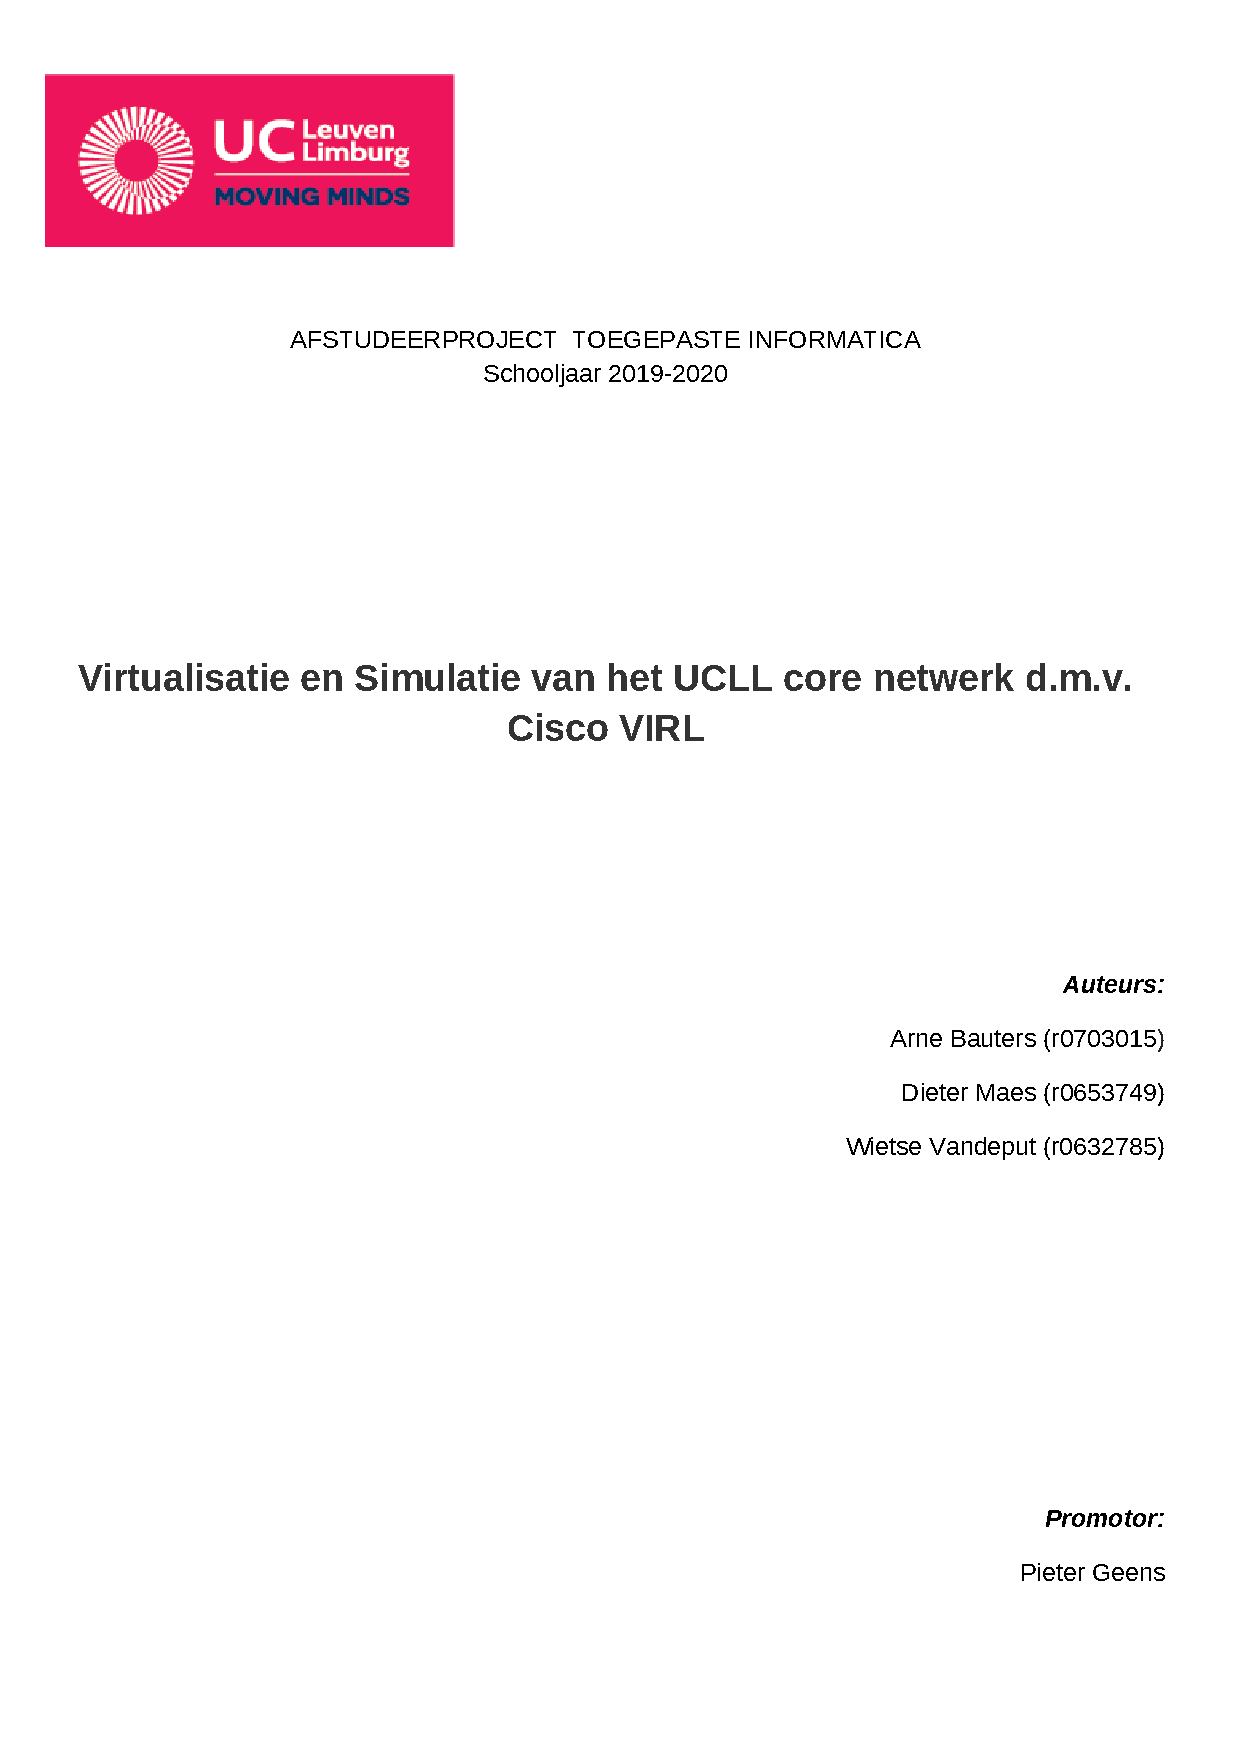
\includepdf[pages=-]{voorblad.pdf}

% \maketitle
% \newpage
\tableofcontents
%\setcounter{tocdepth}{5}

\newpage
\section{Intro}
\subsection{Assignment}

\subsubsection{Original assignment}	
Our assignment was to virtualise/simulate the UCLL core network using Cisco VIRL.
With this virtualized setup, changes can be tested before being pushed to production.
We were asked whether VIRL could be a viable solution to get a test environment, or not.
The goal is to get a working network
- using technologies like VRF Lite, BGP, OSPF, QoS - in VIRL.

\subsubsection{Concrete guidelines}	
Like always the assignment diverts slightly from expectations.
After a couple of sessions with Pieter Geens we defined our scope as following:

We are to research VIRL, it's possible limitations as to virtualise the network and the pro's and con's of the free online Cisco DevNet versus the payed license for running it on own hardware.
The research has to be documented so those willing to use VIRL at the UCLL can easily start doing work instead of figuring out how to use VIRL.
The best way to research this, is to actually implement (a part of) the core network.
The network diagrams were delivered, together with a lot of information,
so we have everything to deliver an attempt at virtualizing of this network.
This document will thus mainly research how to do certain things like VRF Lite, Etherchannel, multi-area OSPF, etc. in Cisco VIRL.

\newpage
\section{Pre-setup Research}
\subsection{VIRL via DevNet}
The Cisco DevNet sandbox is a free sandbox environment where you can test multiple things, including VIRL.
A closed environment with readily available images for routers, switches, firewalls and servers,
can be reserved for a limited time and with limited resources.
We noticed reserving resources for a couple of hours (enough for a full workday)
was fairly simple and without much waiting
and after a couple of minutes you could connect to your environment trough VPN and have access to multiple simulations.
For reservations longer than one day, with a maximum of one week,
your reservation would be in the queue for a few hours.

We started by testing the main technologies we knew the core network would need:
Etherchannel, OSPF, VRF Lite, vPC, AVA clustering, etc.
We did have some trouble with vPC not working on the nx switches
but resolved it by reserving a different environment that did already have the NX-OSv9K switches included.
Another solution would have been download the image of the NX-OSv9K switch online 
and import it in the Web interface.
(More over adding images later in section \ref{sec:adding_images})

\subsection{Alternatives to VIRL}
Aside from the comparison between the free, online, Cisco DevNet sanbox
and the paid license for the less-limited self-hosted variant of VIRL,
we also made the comparison with a few other platforms.

\subsubsection{dCloud}
dCloud is an alternative to Cisco DevNet and the paid license,
that is also online and free, like Cisco DevNet.
It does not require you to reserve your environment,
but this comes at the cost of a more limited environment.
We were only able to use up to 2 machines, which made it pretty useless in our case.

\subsubsection{GNS3}
GNS3 is an open-source solution to the whole VIRL platform.
It is also not vendor-specific.
However, we were not able to quickly find free images for Cisco networking gear.
(they need to be imported, since GNS3 being open-source and vendor-unspecific means they can not provide free images from vendors)
Combined with statements that GNS3 had some troubles with Layer2 functionality in the past,
and the uncertainty if they had already been fixed,
we decided to not further explore this option.

If we had images available this could have been a great alternative,
provided that Layer2 functionality is better than in the past.

\newpage
\section{VIRL Web interface user guide}
\subsection{Cisco DevNet specific instructions}
\subsubsection{Cisco DevNet Webservice}
The webservice provides free resources and a free VIRL test environment,
but it comes with some limitations:
\begin{itemize}
	\item You will be limited in the amount of machines you can use (only 12).
	\item You will have to reserve the resources, with your reservation being limited in time.
		(They do however state you can contact support to extend your reservation, if needed)
\end{itemize}

\url{https://devnetsandbox.cisco.com}

\subsubsection{Login to Devnet}
Obviously, a login is required.
Luckily some options for sign-on with external providers as well as other Cisco services is available.
\begin{figure}[H]
	\centering
	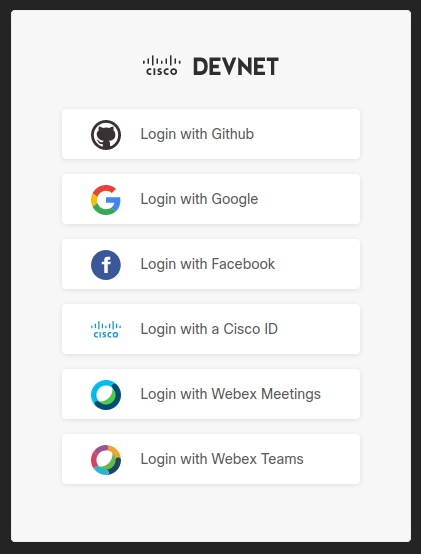
\includegraphics[height=250px]{images/login_to_devnet.png}
\end{figure}

\subsubsection{The Devnet sandbox labs}
The environment offers a lot of services,
but the scope of this project limits us to the VIRL sandbox.
To get this specific sandbox running you have to search the sandbox labs page for either "VIRL" or "Multi-IOS Cisco Test Network".
This page already provides a lot of information on how to use the sandbox,
even more is given by mail once you reserve the resources.
To do this you will have to click \textit{reserve} in the upper-left corner.

\begin{figure}[H]
	\centering
	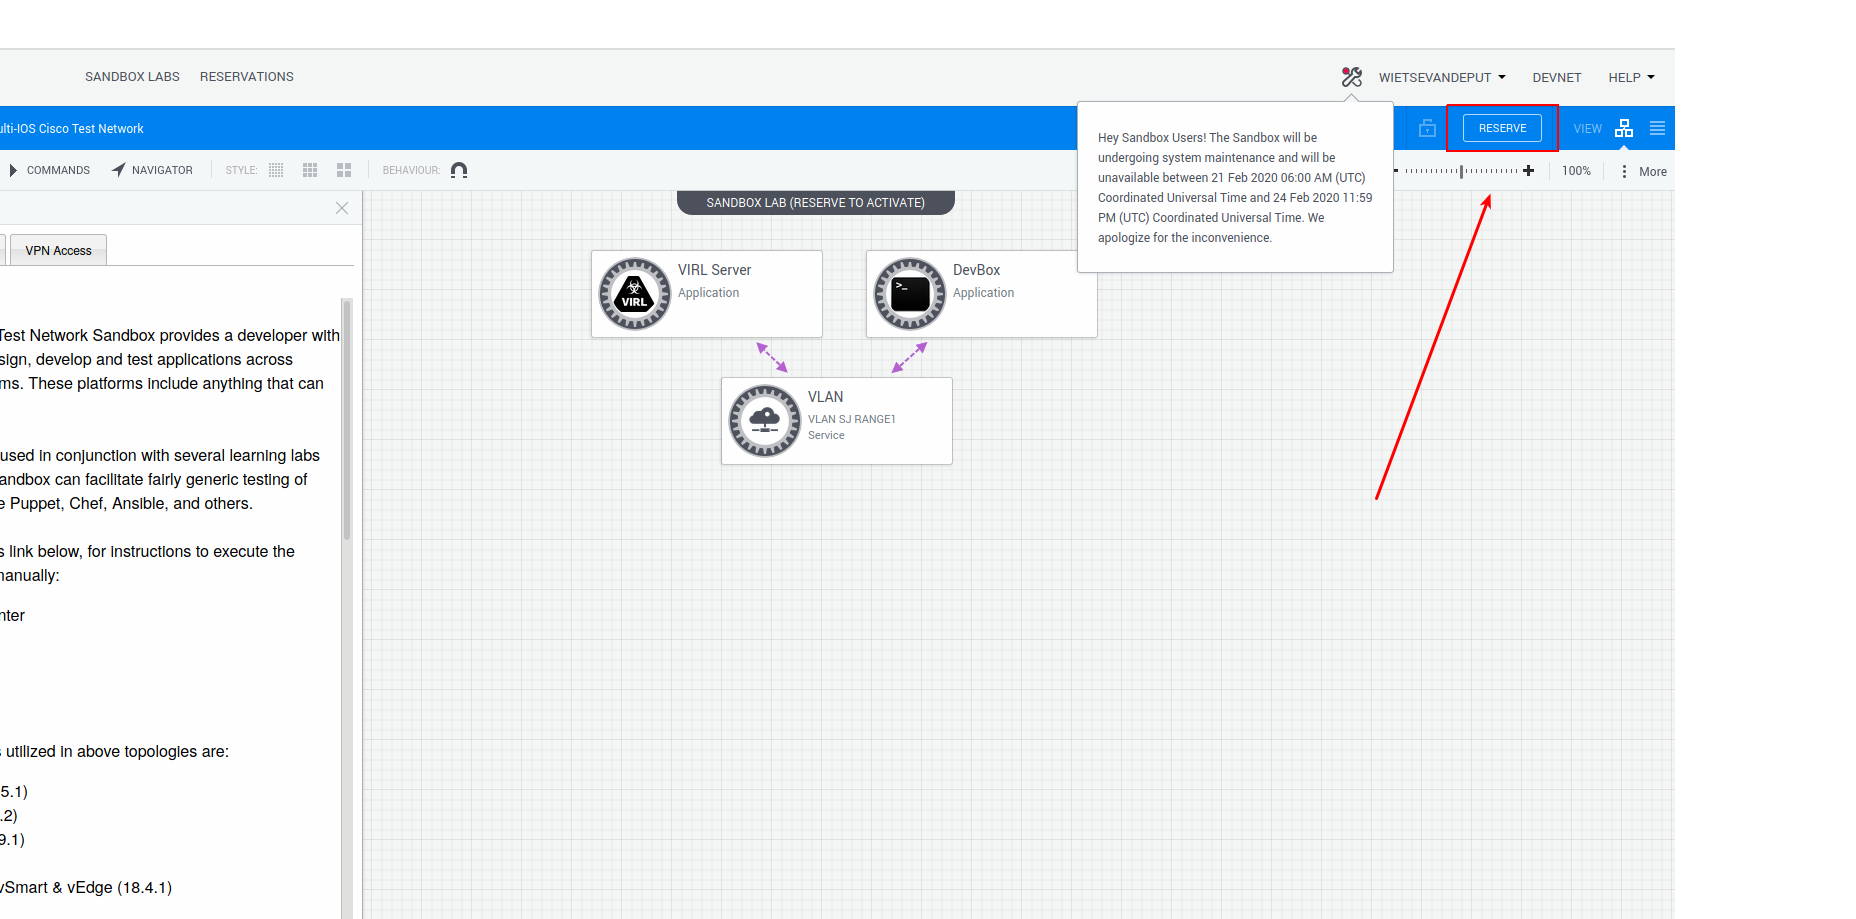
\includegraphics[width=\textwidth]{images/Devnet_Sandbox_VIRL.png}
\end{figure}

\subsubsection{Reserving resources}
In the reservation screen you can define a couple of things:

\begin{description}
	\item[Schedule] Define for how long you would like to reserve your test environment.
		The longer you would want to keep your reservation,
		the longer it will take before there is a slot available and the resources are reserved.
	\item[Name] This very self-explanatory, you can give your sandbox a custom name.
	\item[Sandbox Lab] You can still change what sandbox you would like to use.
	\item[VIRL Simulation] Here you can choose to already start a predefined simulation,
		or just start with a clean slate ("none")
\end{description}

\begin{figure}[H]
	\centering
	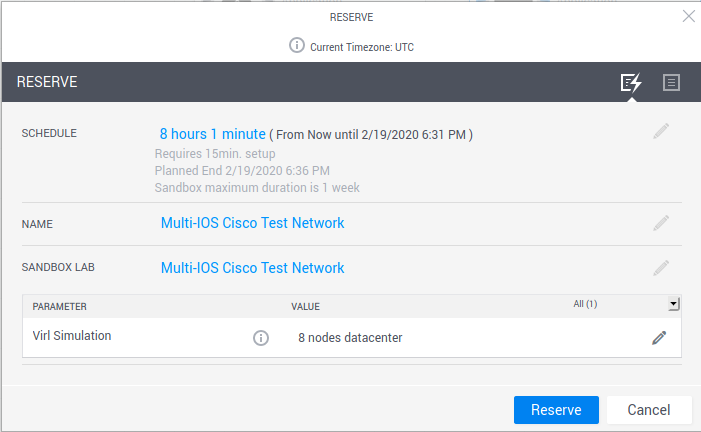
\includegraphics[width=\textwidth]{images/Reserve_resources.png}
\end{figure}

There are also a couple of advanced settings like "owner" and "description" for optimal customization.

\subsubsection{Mails after reservation}
After reserving the resources and the sandbox environment you will receive 2 mails.
One telling you they are currently setting up te sandbox and the time they expect it to take.
Also informing you that you need to connect to it with a VPN.
For Windows they provide a link to their free AnyConnect VPN Client, on Linux you will need to use OpenConnect.

\begin{figure}[H]
	\centering
	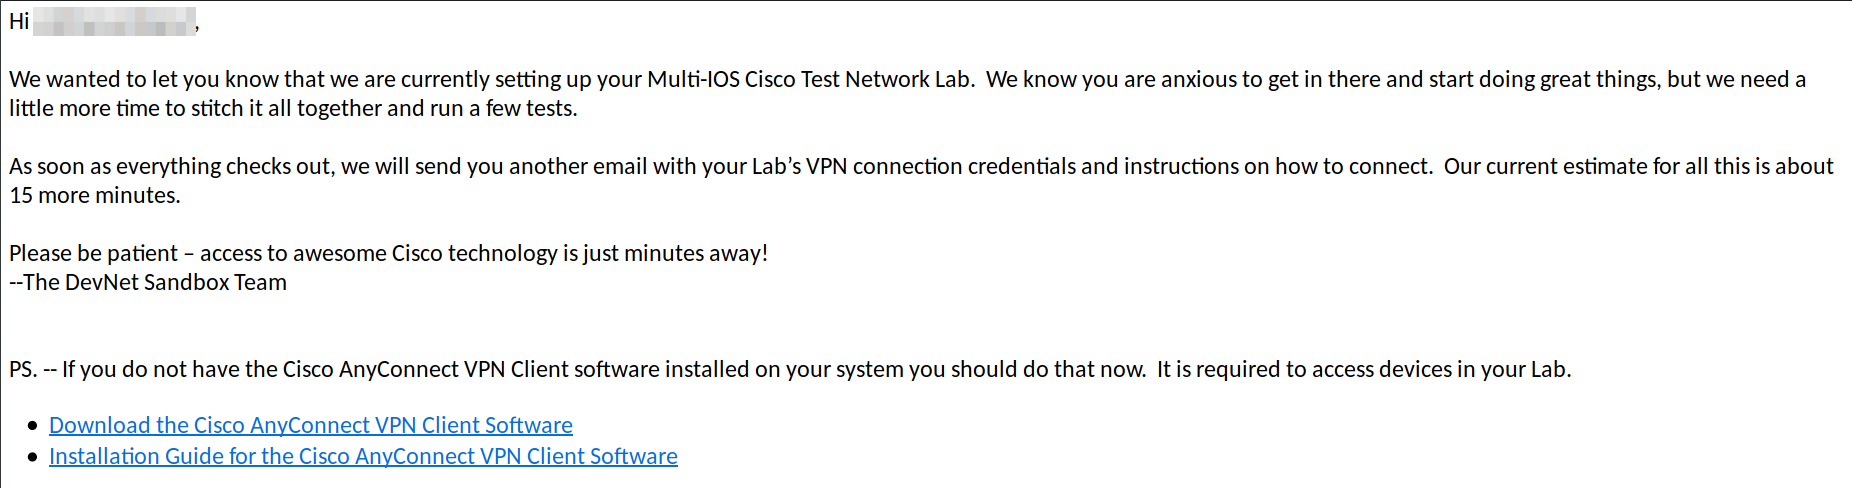
\includegraphics[width=\textwidth]{images/First_mail.png}
\end{figure}

The full Linux command is
\begin{lstlisting}
sudo openconnect --script /usr/share/vpnc-scripts/vpnc-script LAB_ADDRESS
\end{lstlisting}
The \textit{LAB\_ADDRESS} will be provided in the next mail,
together with the username and the password you will be asked for.

\begin{figure}[H]
	\centering
	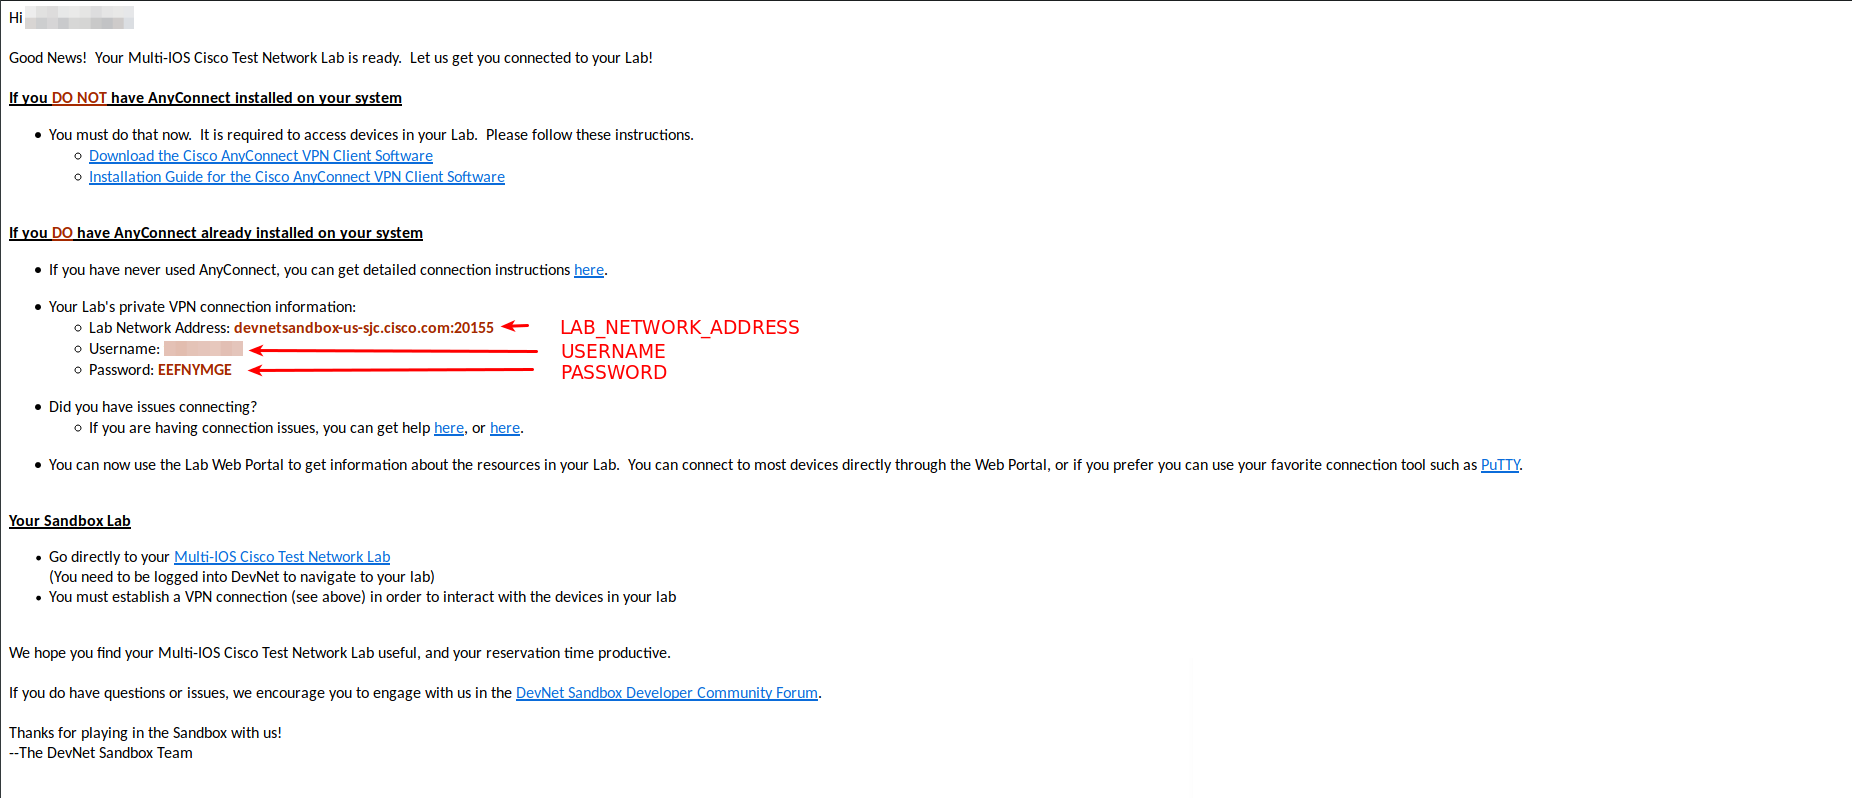
\includegraphics[width=\textwidth]{images/Second_mail.png}
\end{figure}

With these you can connect to the VPN and through that to \url{http://10.10.20.160} in your browser of choice.
You will arrive in the sandbox overview and from here on,
there is little to no difference between the VIRL environment provided by DevNet and the VIRL PE.

\subsection{The Web Interface}
As explained earlier from now on the use of the Web interface will be the same for both the self-hosted VIRL PE and the free DevNet Solution.

\subsubsection{Overview}
When connected to the VIRL Server you can navigate to the UWM (User Workspace Management) page.
This will be your Web interface where you will be able to do all your virtualization and monitoring.

On the left side you find a couple of tabs:

\begin{itemize}
	\item The "Overview" page will give you a representation of the resources available, the resources being used and a quick overview of your active simulations.
	\item The "My Simulations" page will be fully dedicated to your simulations. You get an overview of all the active simulations and resource usage of specific users.
	\item The "Project Simulations" and "Projects" display the projects and their simulations (obviously). Projects get created and named after users automatically. Each User has a password and a role within the project.
	\item The "Users" page is quite self-explanatory and thus displays all the users on the server.
	\item The "VIRL Server" page is where you can update your license, find some tools and downloads.
	\item The "Connectivity" tab gives you information about the network and how to connect to certain projects.
	\item The "VM Control" page gives you all the information about every node, network, connection, host and port currently being virtualized on the server.
	\item The "Node Resource" page will give you all information about the different nodes you can use in the virtualization. Information about the images, etc.
	\item The "Repository" page gives you the option to connect to a GIT repository.
	\item The "Documentation" and the "Community" pages are for additional information either provided by the developers or the community.
\end{itemize}

\begin{figure}[H]
	\centering
	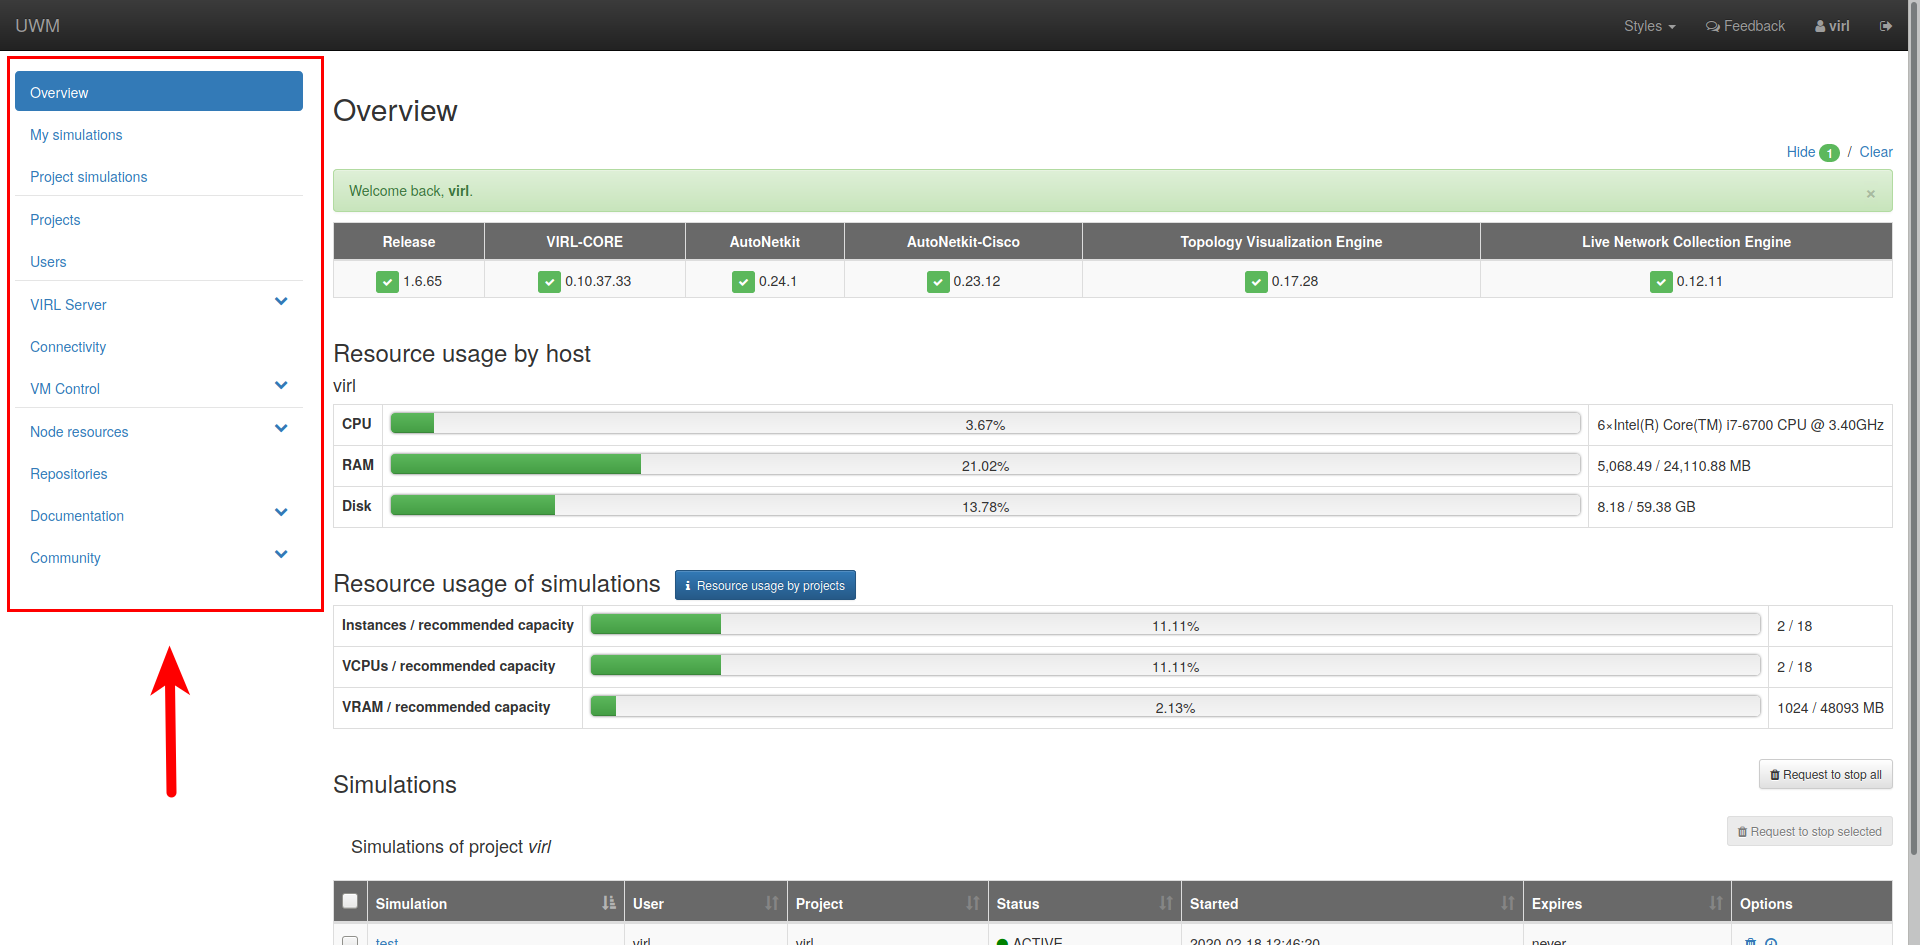
\includegraphics[width=\textwidth]{images/UWM_Overview.png}
\end{figure}

\subsubsection{Make a simulation}
To launch a new simulation is actually very easy and rather fast. Start by clicking the "Launch new simulation" button on the "Simulations" page.\\

\begin{figure}[H]
	\centering
	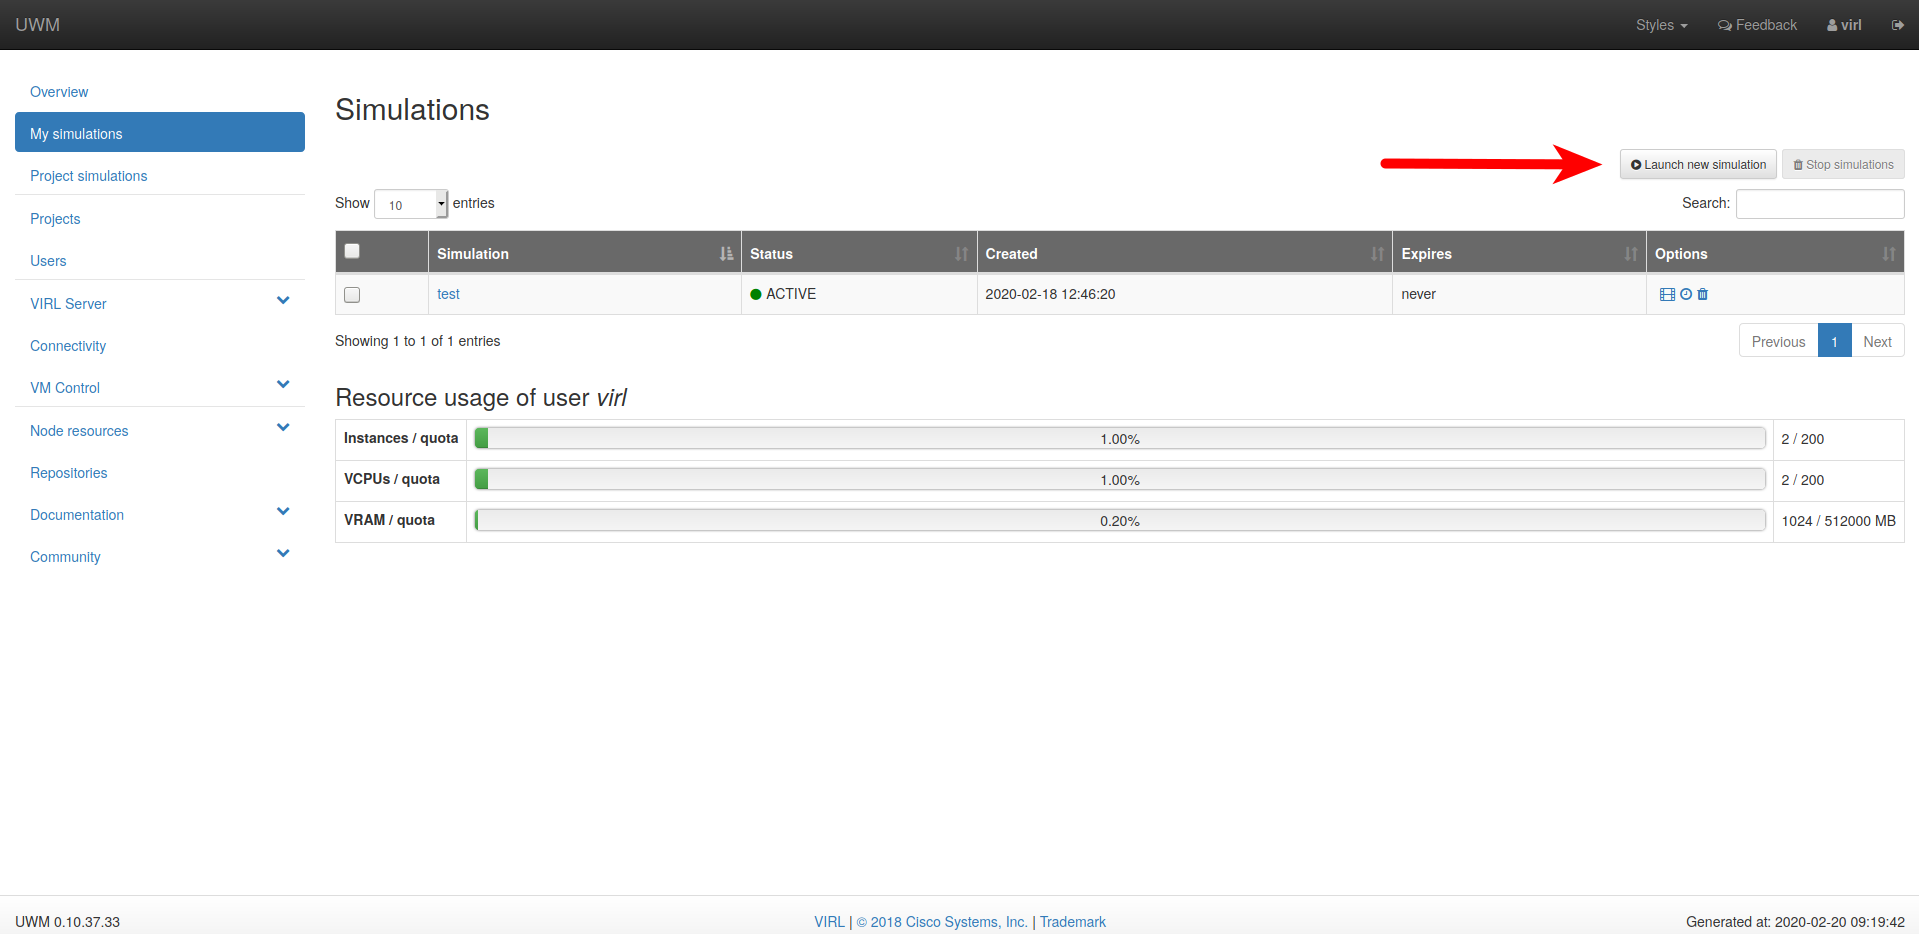
\includegraphics[width=\textwidth]{images/Launch_new_simulation.png}
\end{figure}

Each simulation will take up resources as long as they are active.
As far as we know there is no option to disable them other than to stop them completely.
If you are done with one simulation we thus advise to get the full configuration file as well as the original .virl file and save them either locally or on git.
You will be able to re-simulate already existing .virl files very easily.

Next you will have to choose the source of the simulation:
\begin{description}
	\item[Local .virl file:] You can use this if you already have a .virl file that you want to launch.
	\item[Remote .virl file:] You can also simulate .virl files that are accessible either via HTTP or from a git repository.
	\item[Editor:] This one is not so clearly stated but you can also make a new .virl file in the editor. To do this you have to click the "editor" button, this will bring you to the VIRL editor (more of this in the next section).
\end{description}

\begin{figure}[H]
	\centering
	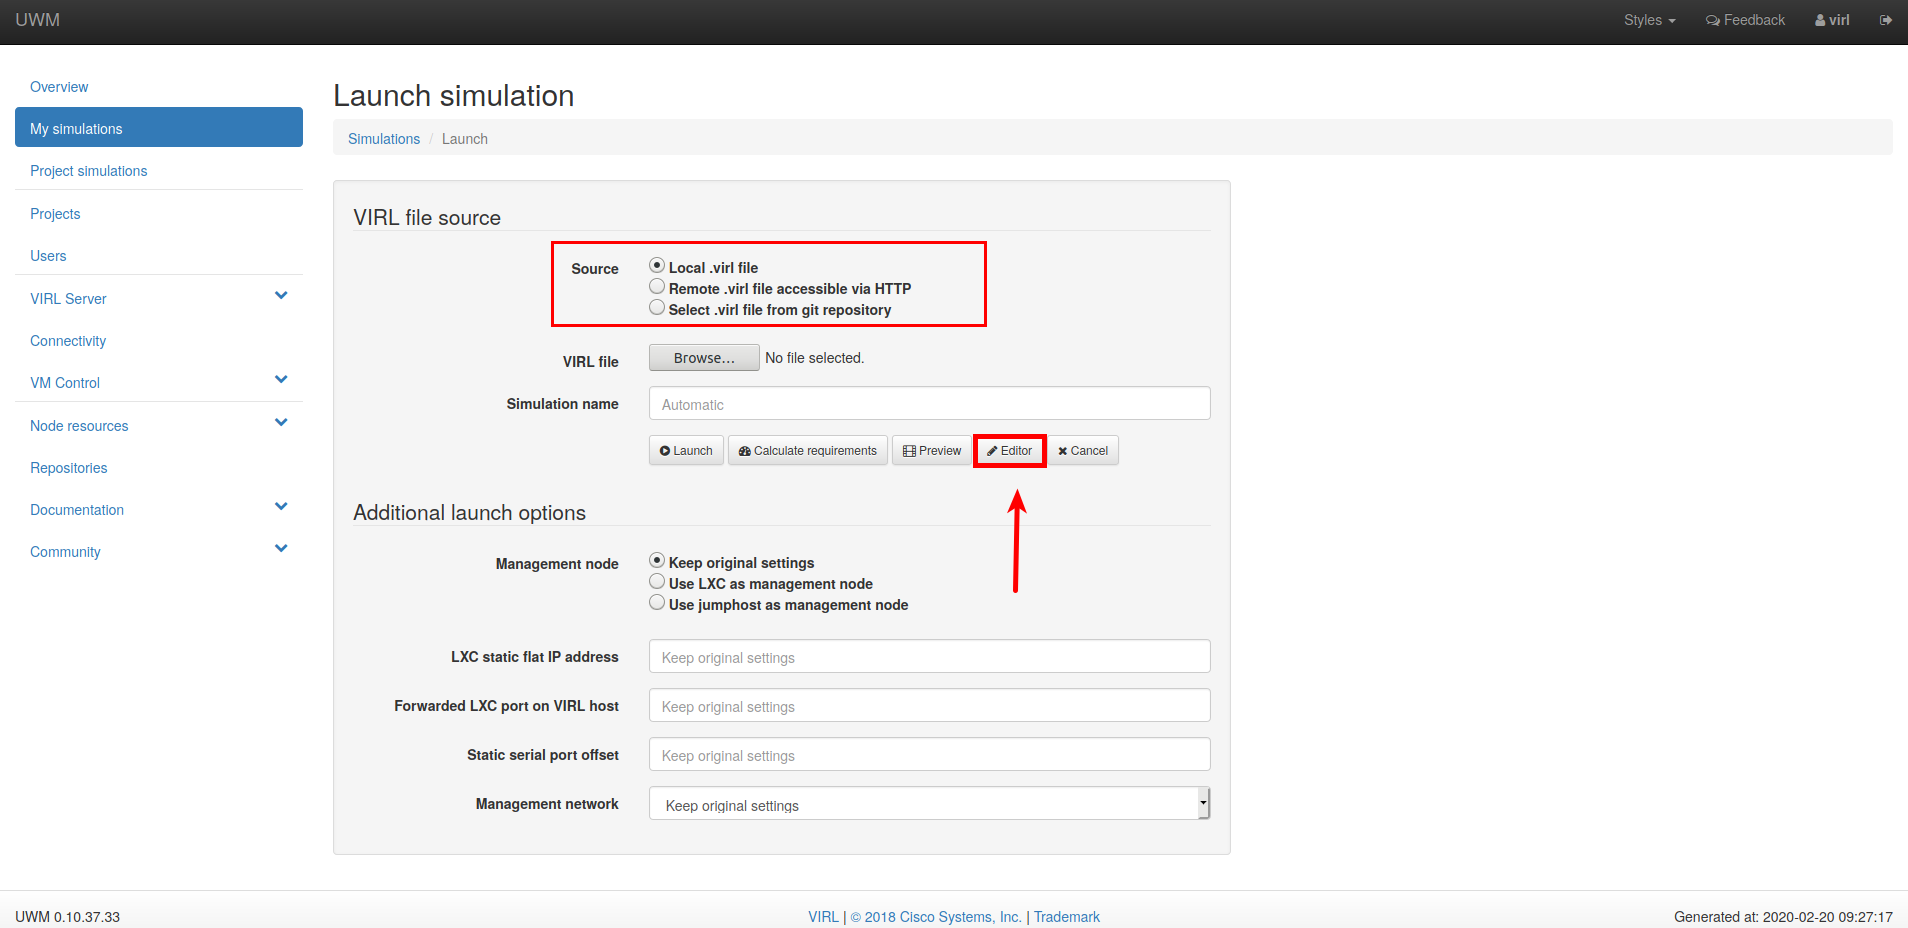
\includegraphics[width=\textwidth]{images/Simulation_config.png}
\end{figure}

Now that you have chosen a source for your simulation all you have to do is to give it a name and launch it.\\
There are some additional launch options you can edit but we have little information about this as we didn't need any alterations for these.

\subsubsection{The VIRL editor}
\begin{figure}[H]
	\centering
	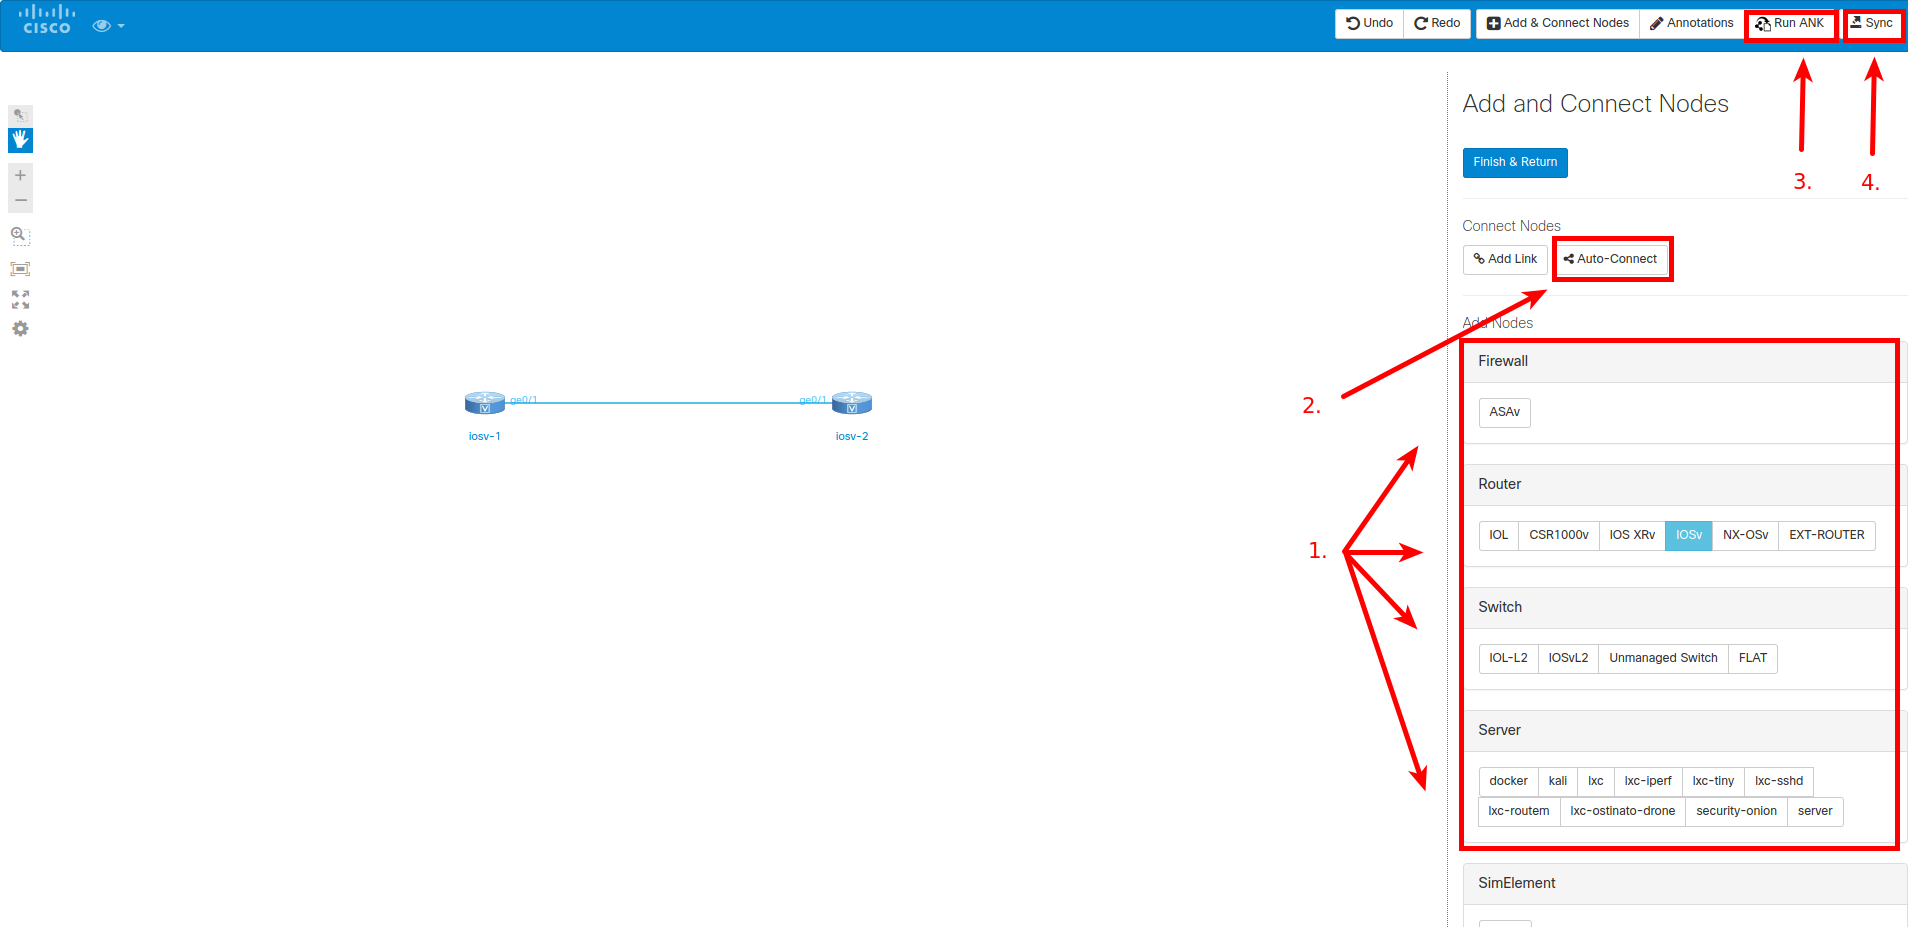
\includegraphics[width=\textwidth]{images/Editor.png}
\end{figure}

\begin{enumerate}
	\item Here you can find all different nodes to add to you topology. Just select the node you want to add and click anywhere in your editor to place.
	\item You can add links manually but you can also auto-connect all devices.
	\item You can run ANK after everything seems to be alright. This will auto configure basic configuration on all devices. This is very useful for tests as you don't have to do the basic configuration anymore. If you like to test everything or don't like basic configuration you do not have to click this for most nodes. If you use a server node anywhere in your topology you are required to push this ANK button otherwise you will not have access to these server nodes.(You can always delete the configuration on the other nodes.) 
	In the next chapter we will cover ANK.
	\item When you are all set you need to push "Sync" in the upper right corner. This will sync the .virl file to the UWM Simulations> Launch new simulation page. there will be a new option by source: "Use .virl file from editor"
\end{enumerate}

\begin{figure}[H]
	\centering
	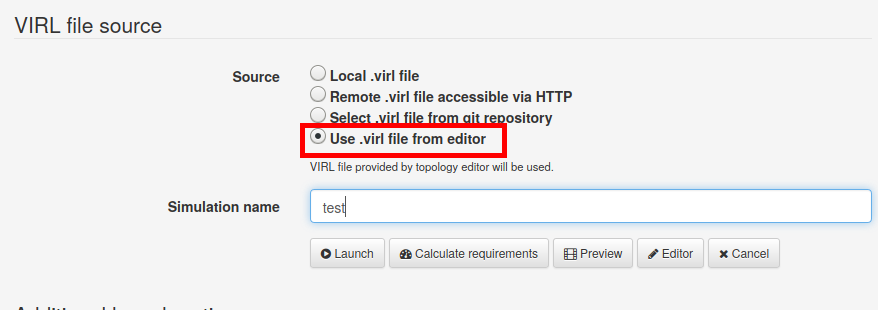
\includegraphics[width=\textwidth]{images/Virl_from_editor.png}
\end{figure}

\subsubsection{Autonetkit ANK}
AutoNetKit is a tool that can configure the network automatically. This is very handy to create a simple configuration for your topology.
It automatically adds protocols, allocates IP addresses and generates configuration files with technologies like BGP, OSPF and many more.

\begin{figure}[H]
	\centering
	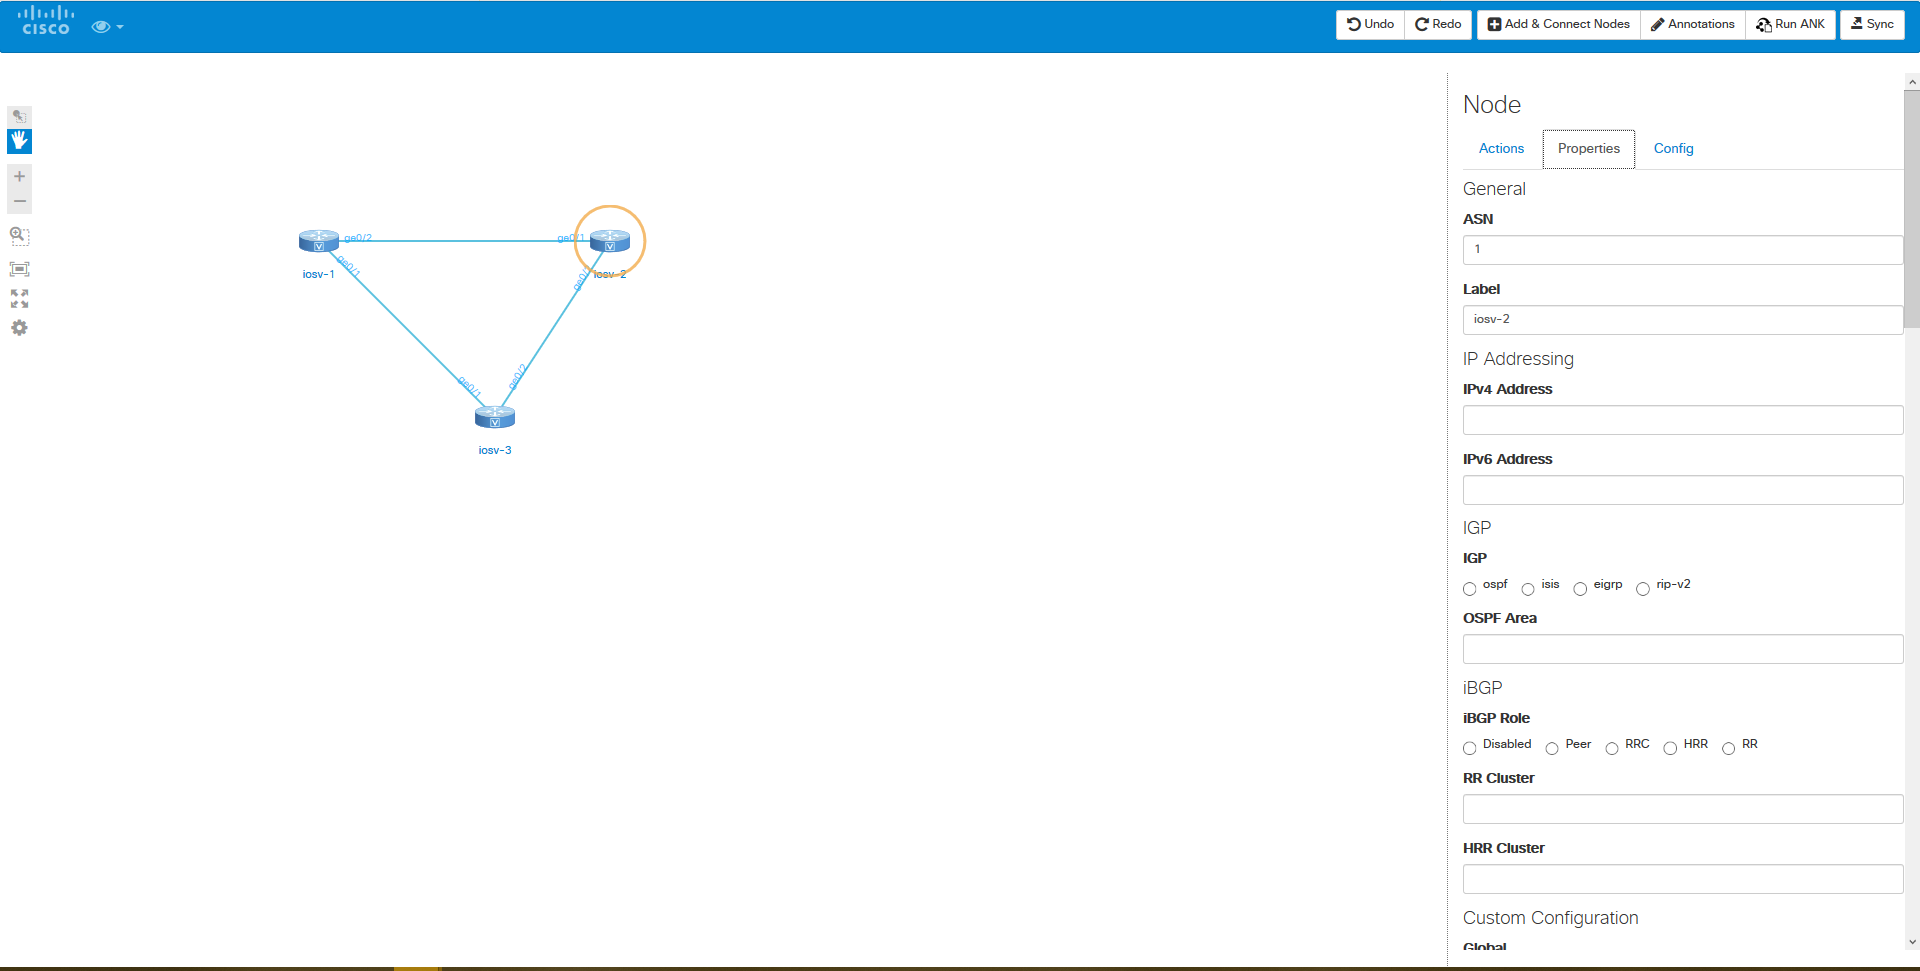
\includegraphics[width=\textwidth]{images/ANK.png}
\end{figure}

When you click on a device like an OSv router and select the properties pane,
you see multiple fields where you can fill in a bunch of properties like the ipv4-address, bgp configuration, OSPF area's \dots
This can also be done for multiple devices at the same time by holding down the SHIFT button while clicking the devices.

When you're done filling in your preferences you can click on ANK in the upper right corner.
Now you can see the config of the device in the config pane.
Here you can also remove parts or edit the configuration to your liking.
However sometimes when you fill in your preferences like ipv4-addresses ANK will override this and not use your configuration.
This often happened in our project.
We ran ANK to get a basic configuration and removed the parts of the config we didn't need or want.

\begin{figure}[H]
	\centering
	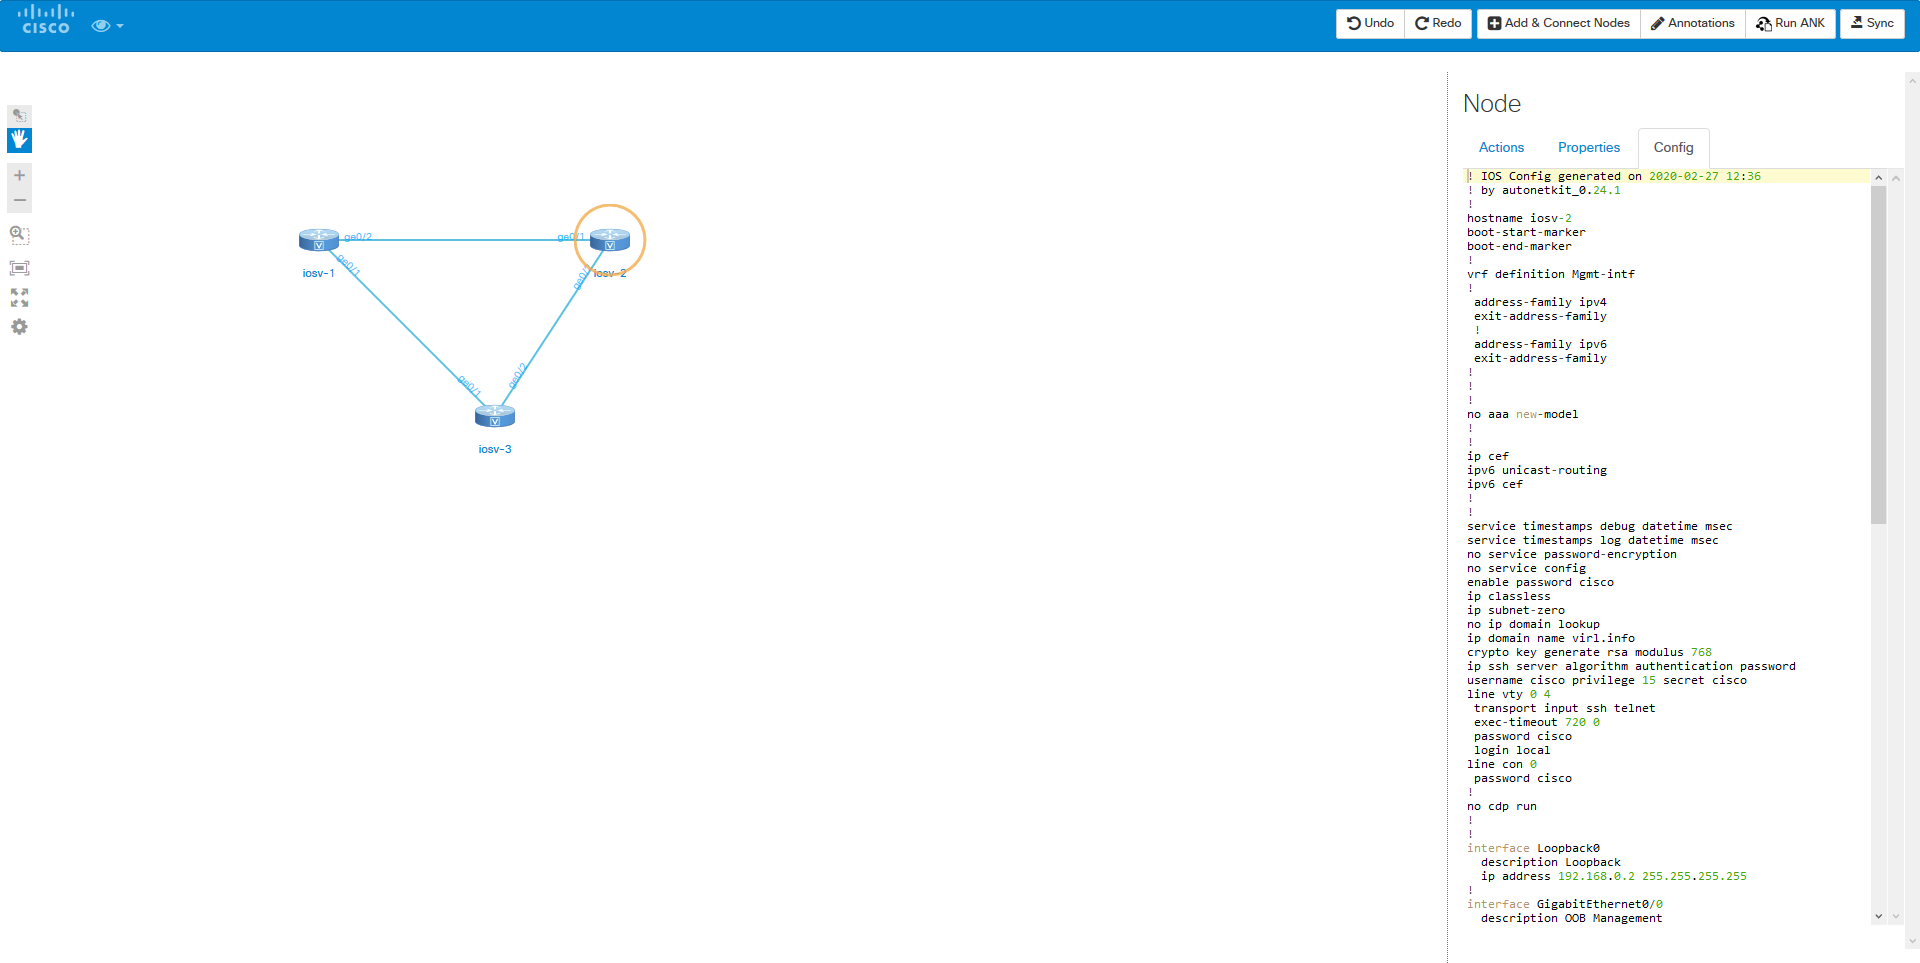
\includegraphics[width=\textwidth]{images/ANK_Config.png}
\end{figure}

When you use servers you are forced to run ANK on these devices, otherwise there are no usernames and passwords configured and you will be unable to gain access to the devices.
This can't be done manually.
We used ANK for creating the basic configuration so we didn't need to manually type the same things over and over again.
Thus saving time for the more complex configurations.

\subsubsection{The Simulation}
Congratulations, you now have made a simulation in the VIRL Web interface.
The nodes will take a moment to initialize but once everything is active and reachable you are able to start playing around with your network.

You will be send to the Simulation "test" details page.
You can get back to this page by going to "My Simulations" and clicking on the simulation you want to view the details of.

On this page you see a number of things, ranging from the nodes overview (with the links and information how to connect to these), traffic captures, interfaces, links and simulation messages.
If you want to start playing around with your network you can connect to any node you want using the telnet commands or you can click "Live Visualization".

\begin{figure}[H]
	\centering
	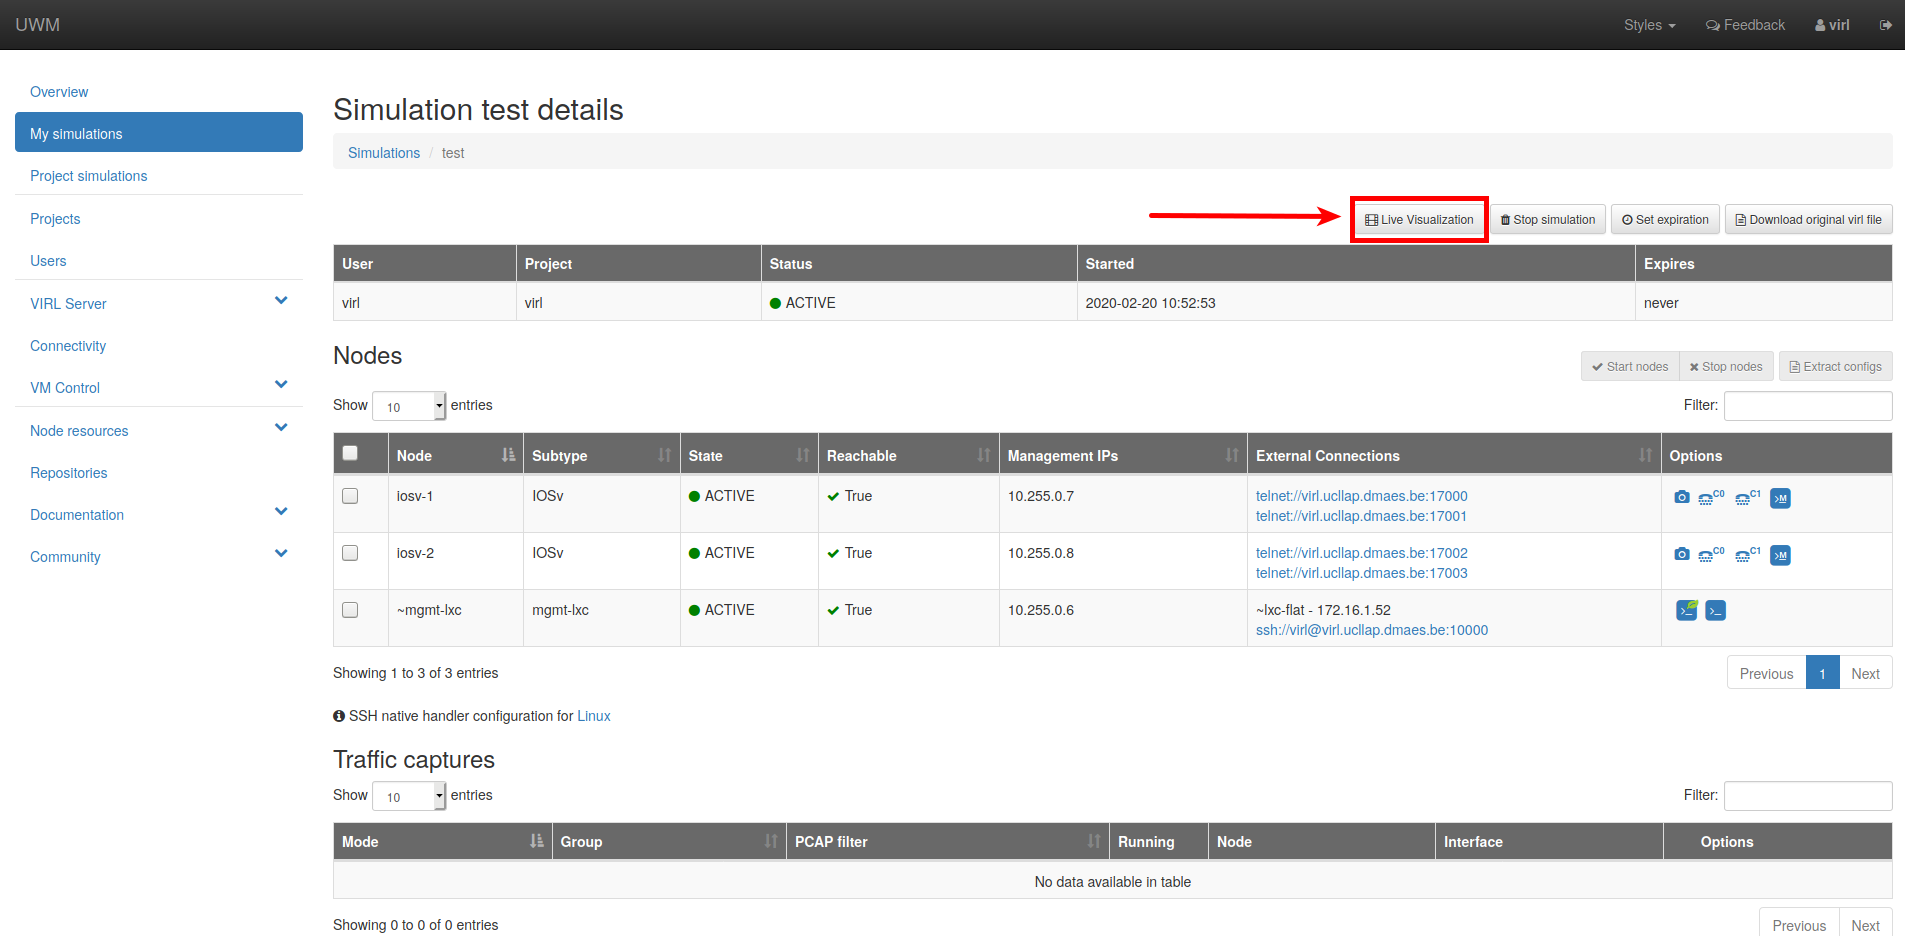
\includegraphics[width=\textwidth]{images/Live_visualization.png}
\end{figure}

\newpage
The AutoNetkit visualization screen allows you to see how all the nodes are connected to each other, you can see the different routing protocols, autonomous system numbers \dots
To use the visualization screen you must have created the topology and generated the config files using the ANK tool.
In this screen you can click any node and connect through telnet to the devices.
From there you can configure them.
You can also connect through the terminal.
When hovering over the nodes a pop-up menu is available from where you can Telnet to the devices, ping from or to the devices \dots

\begin{figure}[H]
	\centering
	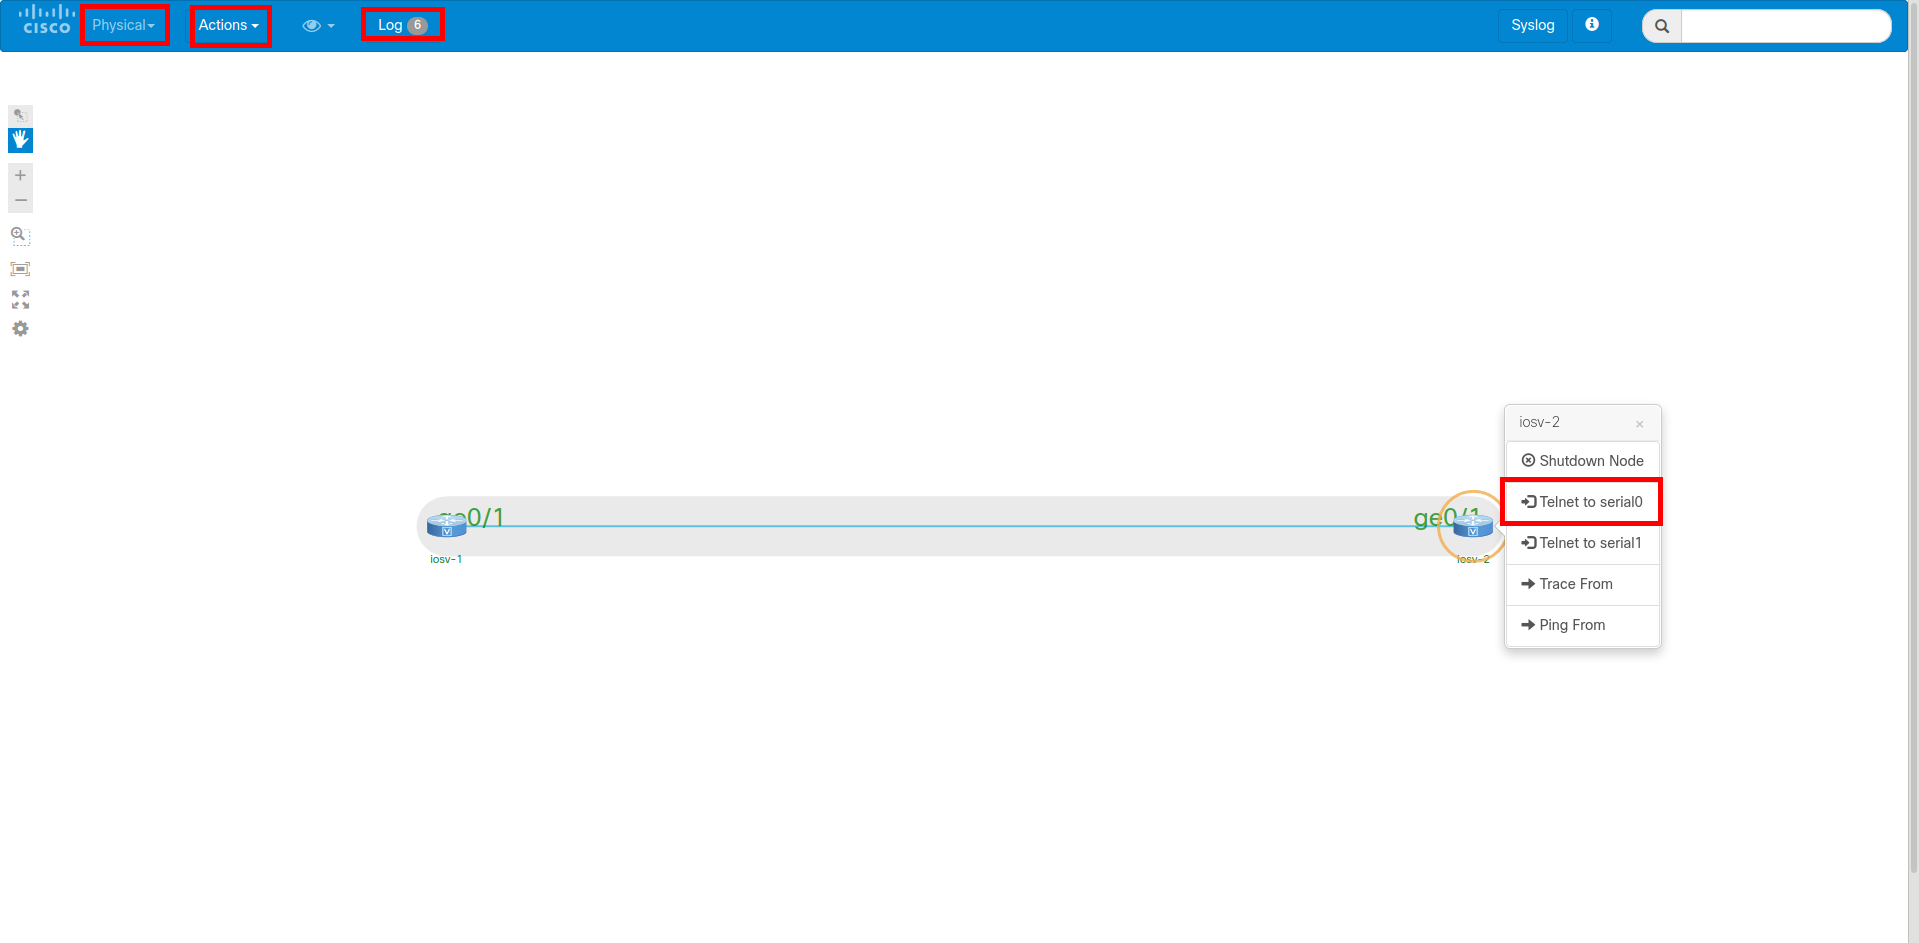
\includegraphics[width=\textwidth]{images/Connect_to_router.png}
\end{figure}

There are a couple of view options for the topology.
The default one showed on the screen is the pysical model of the topology.
This shows the nodes and conncetions between them.
Under "Physical", you can select other options like a BGP, OSPF, Layer one, Layer two or Layer three Views.
The Live visualization also allows you to run a couple of "Actions" to for example collect data or parts of the running-config.
In "Log" you get the results of actions or pings.

\begin{figure}[H]
	\centering
	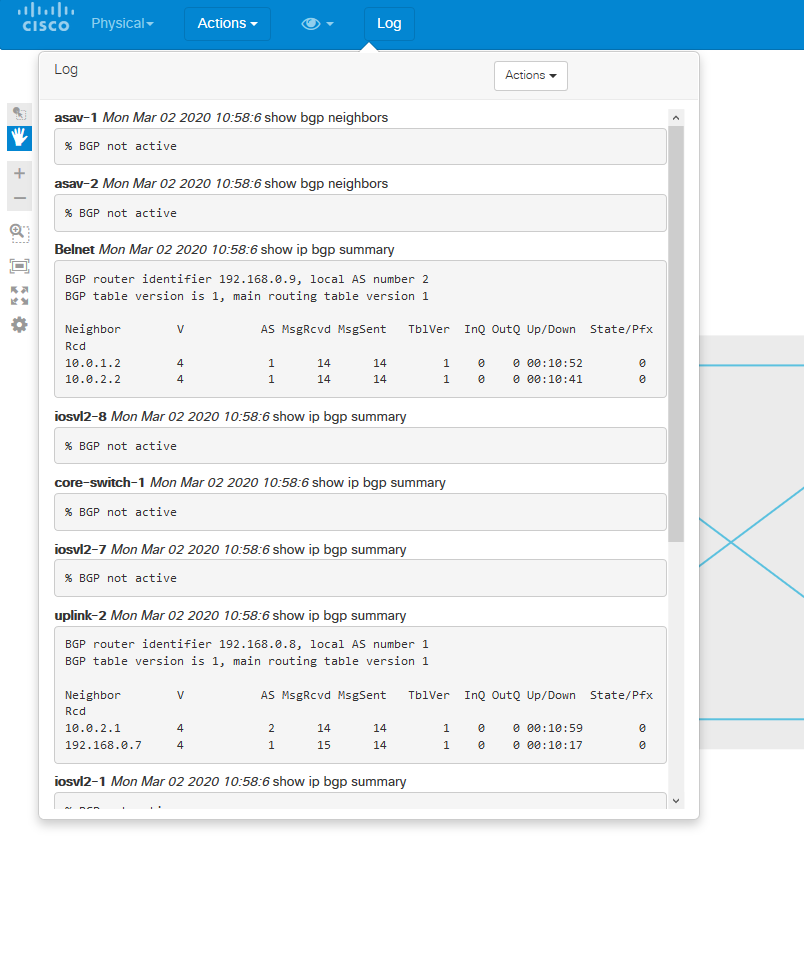
\includegraphics[width=\textwidth]{images/bgp_log.png}
\end{figure}

Here you see all the BGP information from every device of the topology under the "log" tab.

\subsubsection{Save the original .virl file as well as the configured one}
\begin{figure}[H]
	\centering
	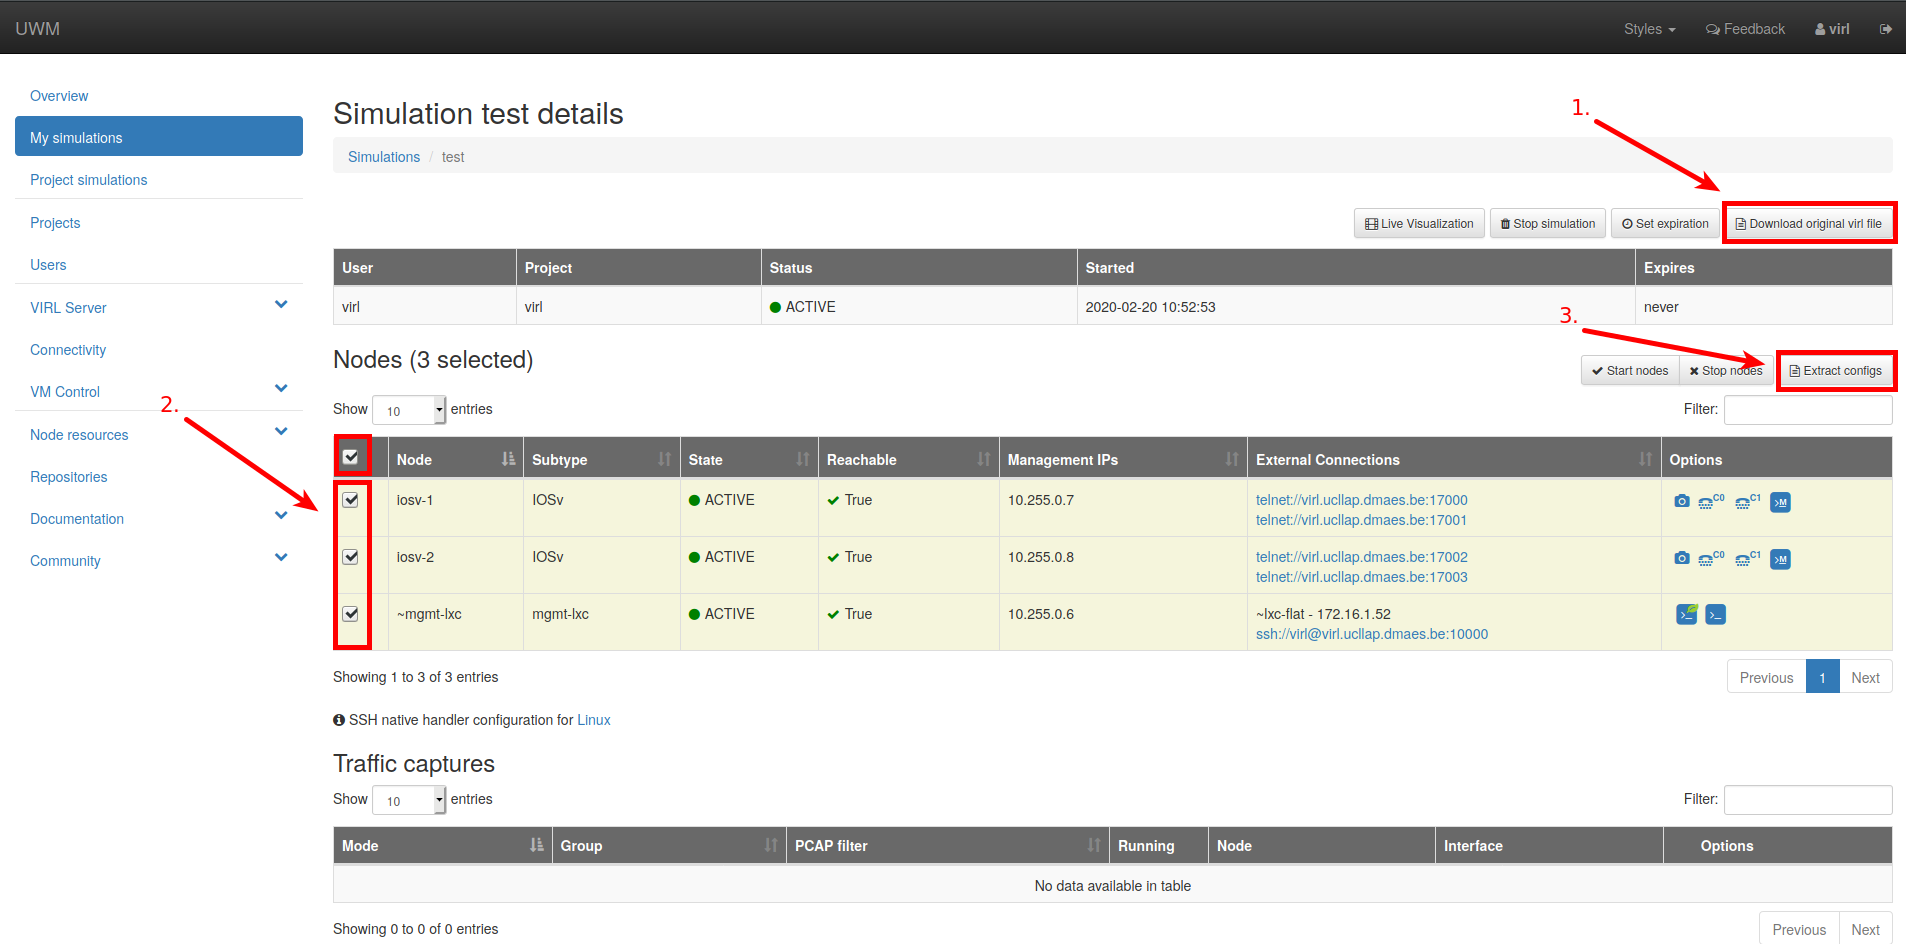
\includegraphics[width=\textwidth]{images/Save_virl.png}
\end{figure}

\begin{enumerate}
	\item If you want to save the original .virl file you can click the button on the top right, this will have only the default configuration if you pressed ANK in the editor.
	\item If you also want to save the configuration you have done in the simulation you can select the nodes from witch you want to save it. 
	\item And press "Extract configs".
\end{enumerate}

\newpage
\subsubsection{Adding a git repository}
There is an option for adding git repositories to the VIRL UWM:

\begin{figure}[H]
	\centering
	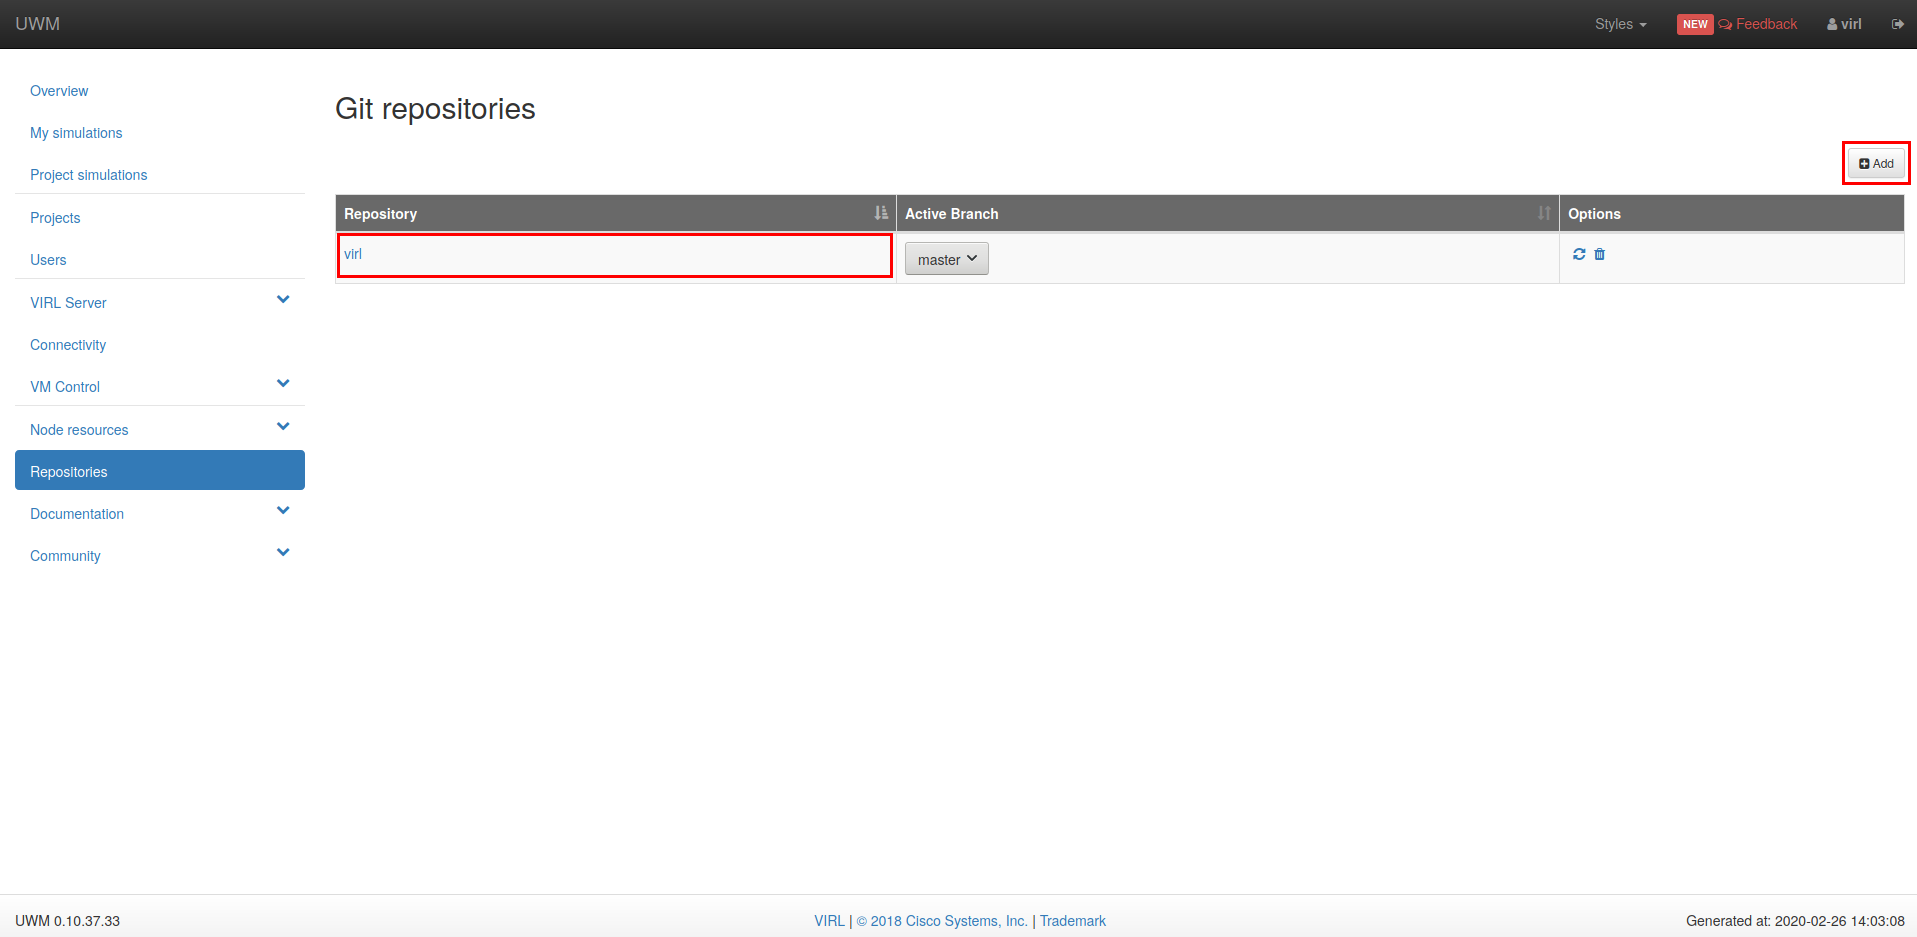
\includegraphics[width=\textwidth]{images/Add_repo.png}
\end{figure}

You can either add a new repository or enter one you already have connected.
We will first take a look at adding one.

\begin{figure}[H]
	\centering
	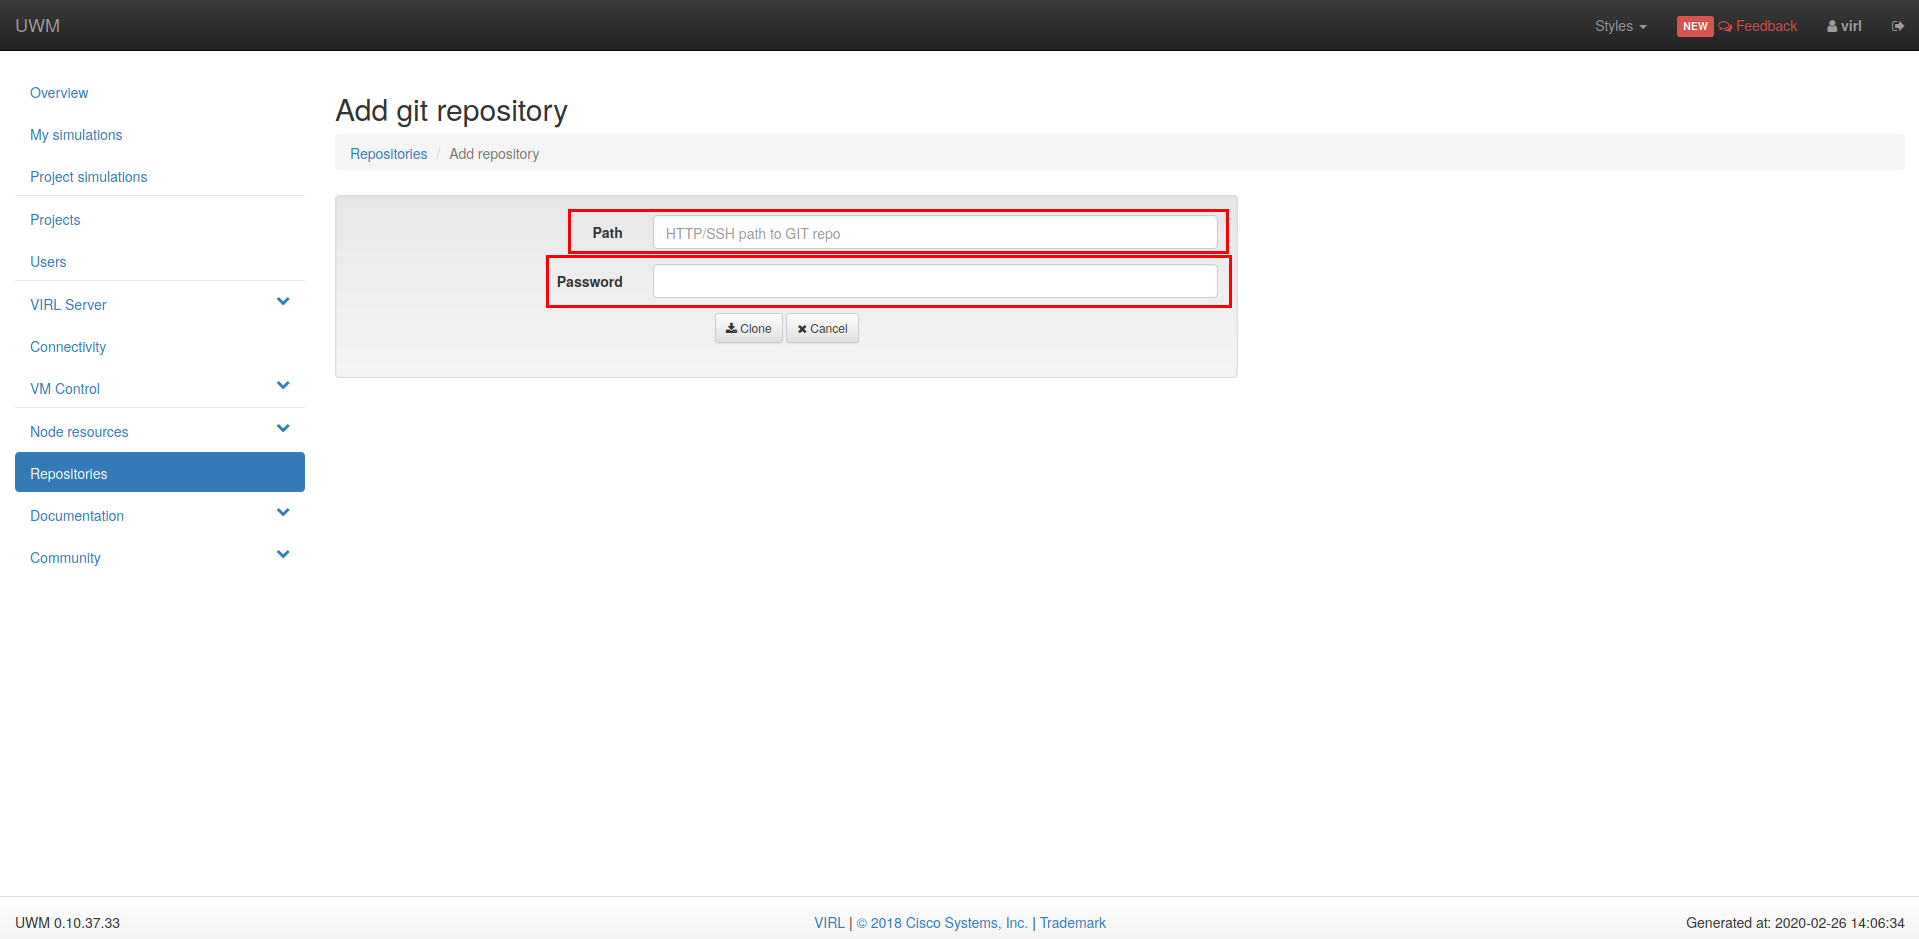
\includegraphics[width=\textwidth]{images/Adding_new_repo.png}
\end{figure}

Here you will have to specify the clone path and the password of the user.
For this to work make a user on your gitlab with the same name as your VIRL user or the other way around make your VIRL user match your gitlab username.

\newpage
When you have added a repository you can enter it and even launch .virl files straight from the repository.

Sadly we have not found an easy way to push to the repository from UWM.
You can manually extract the .virl files and push them yourself as seen in the previous section.

\begin{figure}[H]
	\centering
	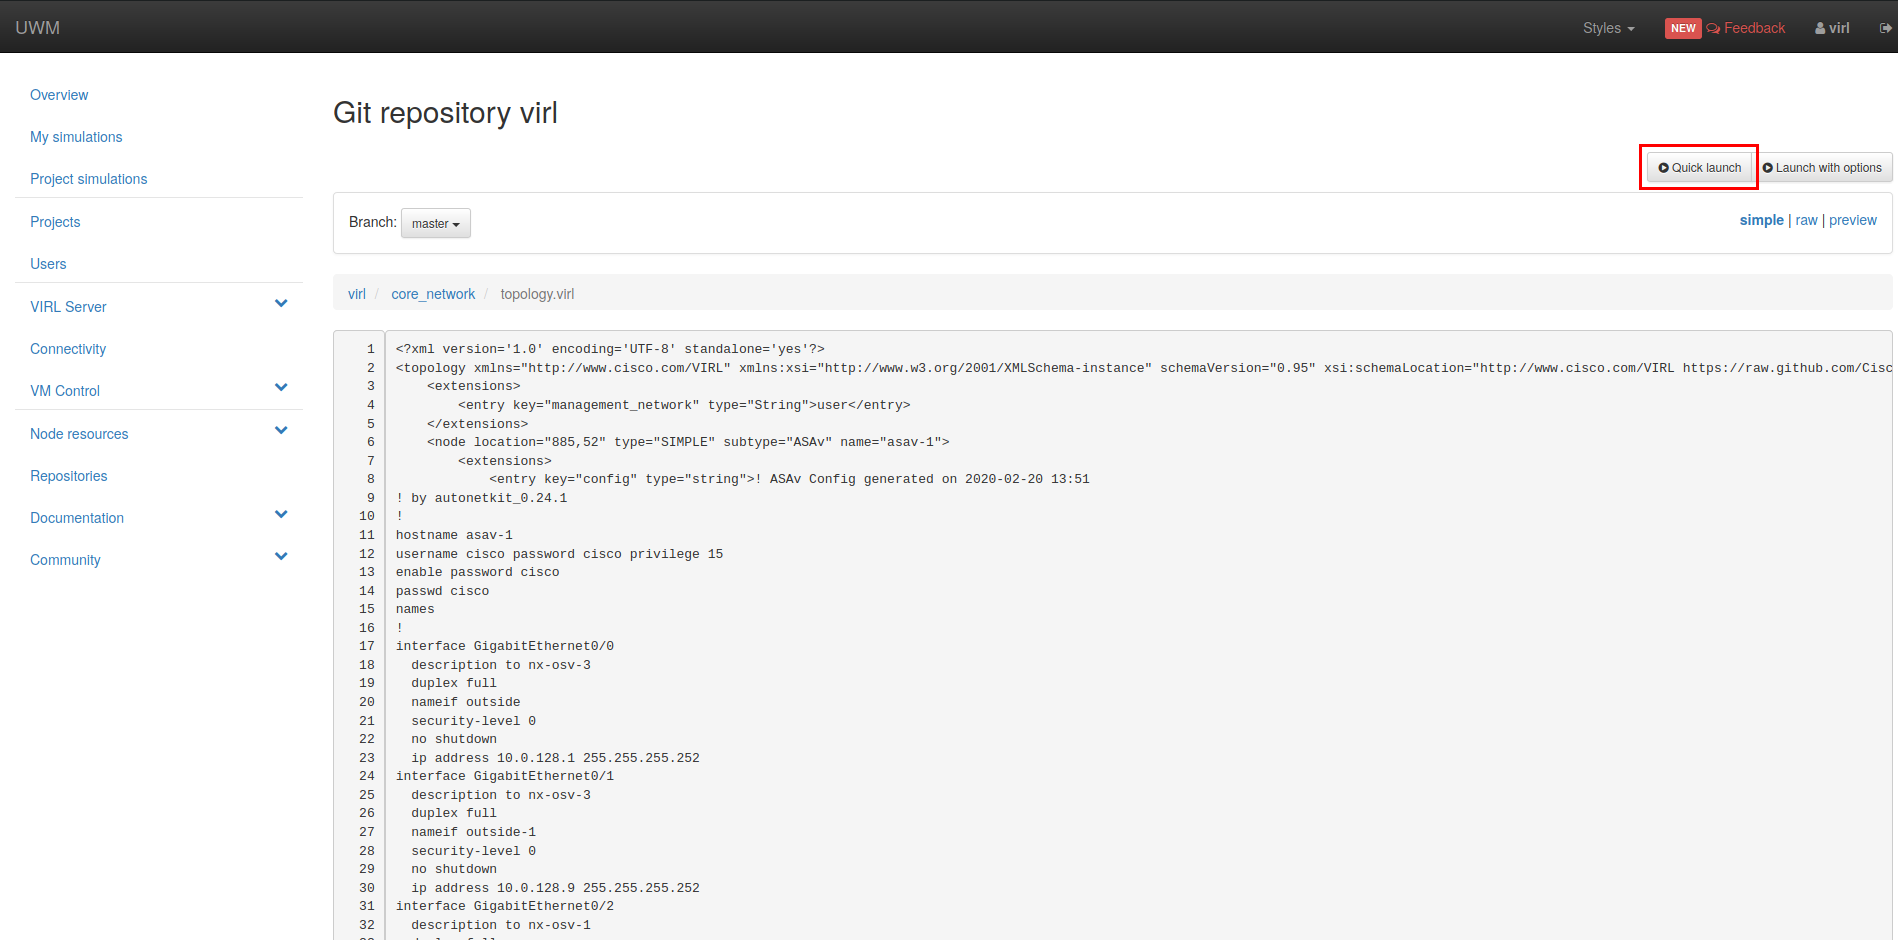
\includegraphics[width=\textwidth]{images/Launch_from_repo.png}
\end{figure}

\subsubsection{Adding images} \label{sec:adding_images}
Earlier we already spoke of having troubles with certain nodes not supporting certain techniques.
As a solution you can look for a different sandbox environment in the Devnet solution,
or if you run your own VIRL server you can also add images or update an existing device with a newer image in the UWM.

Go to the main page and click \textit{Node resources} $rightarrow$ \textit{Images} $rightarrow$ \textit{Add}.

\begin{figure}[H]
	\centering
	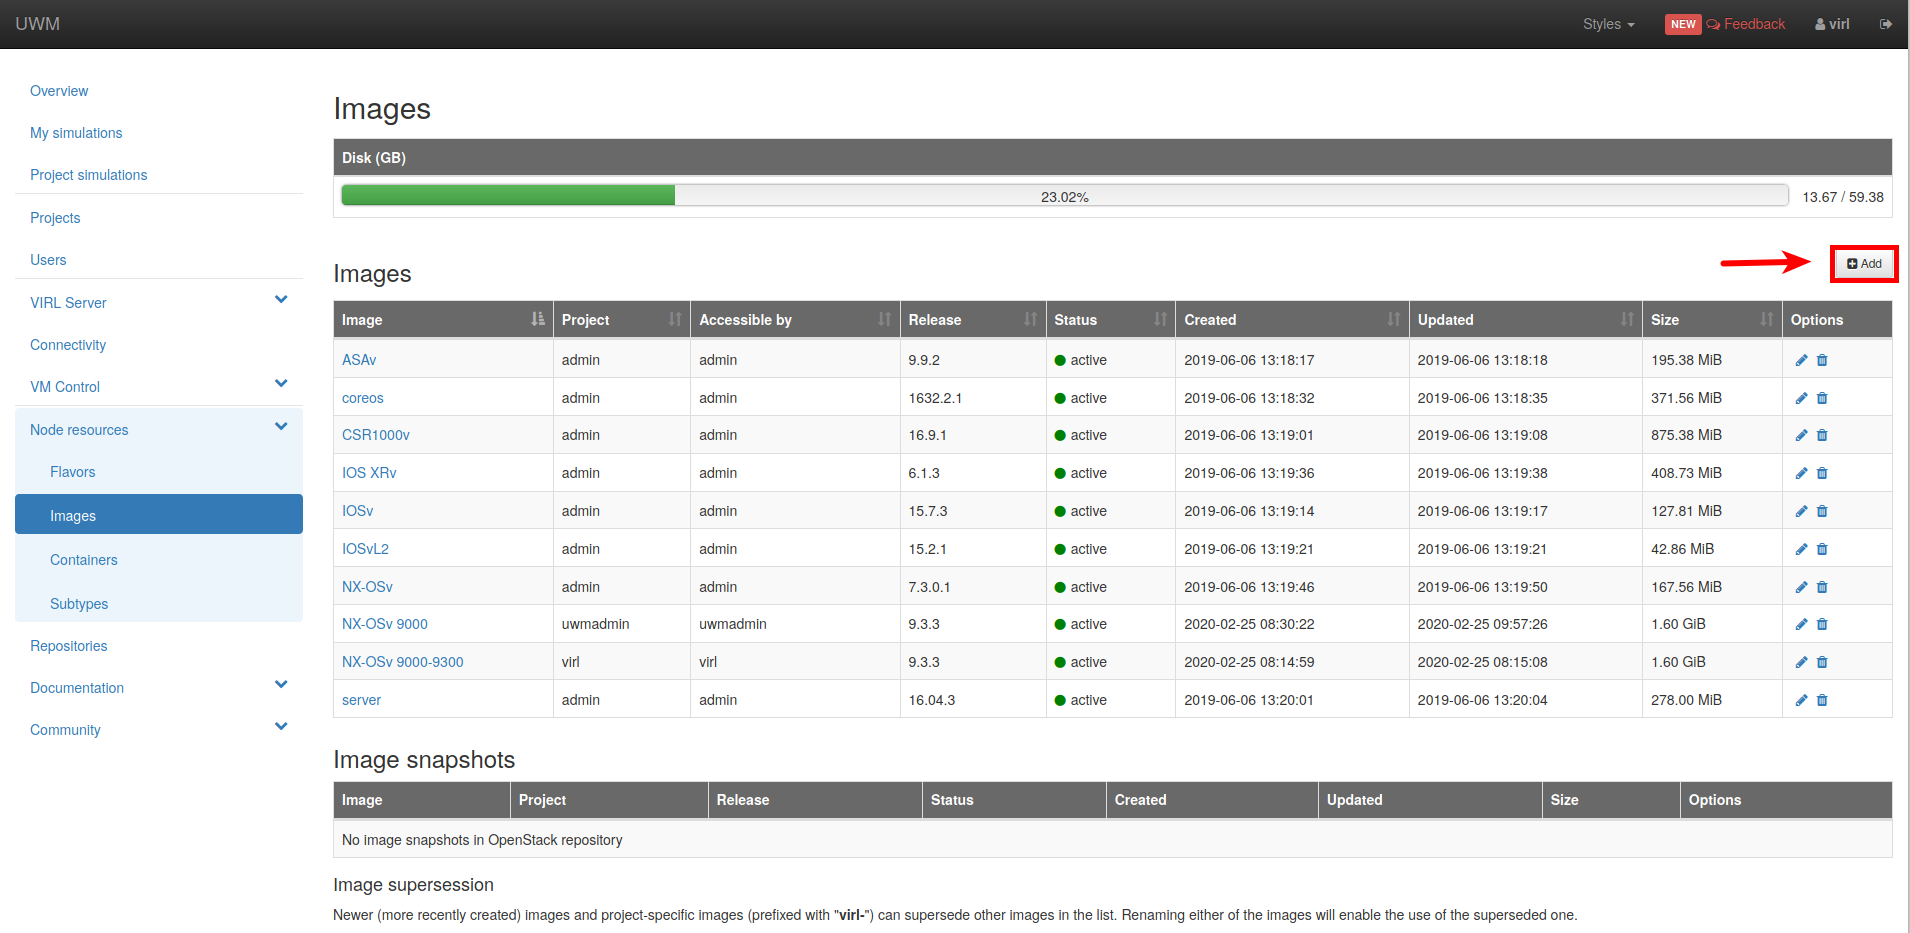
\includegraphics[width=\textwidth]{images/Add_images.png}
\end{figure}

We will use the example of adding the NX-OSv9K since we needed these for our simulation.

\newpage
\begin{figure}[H]
	\centering
	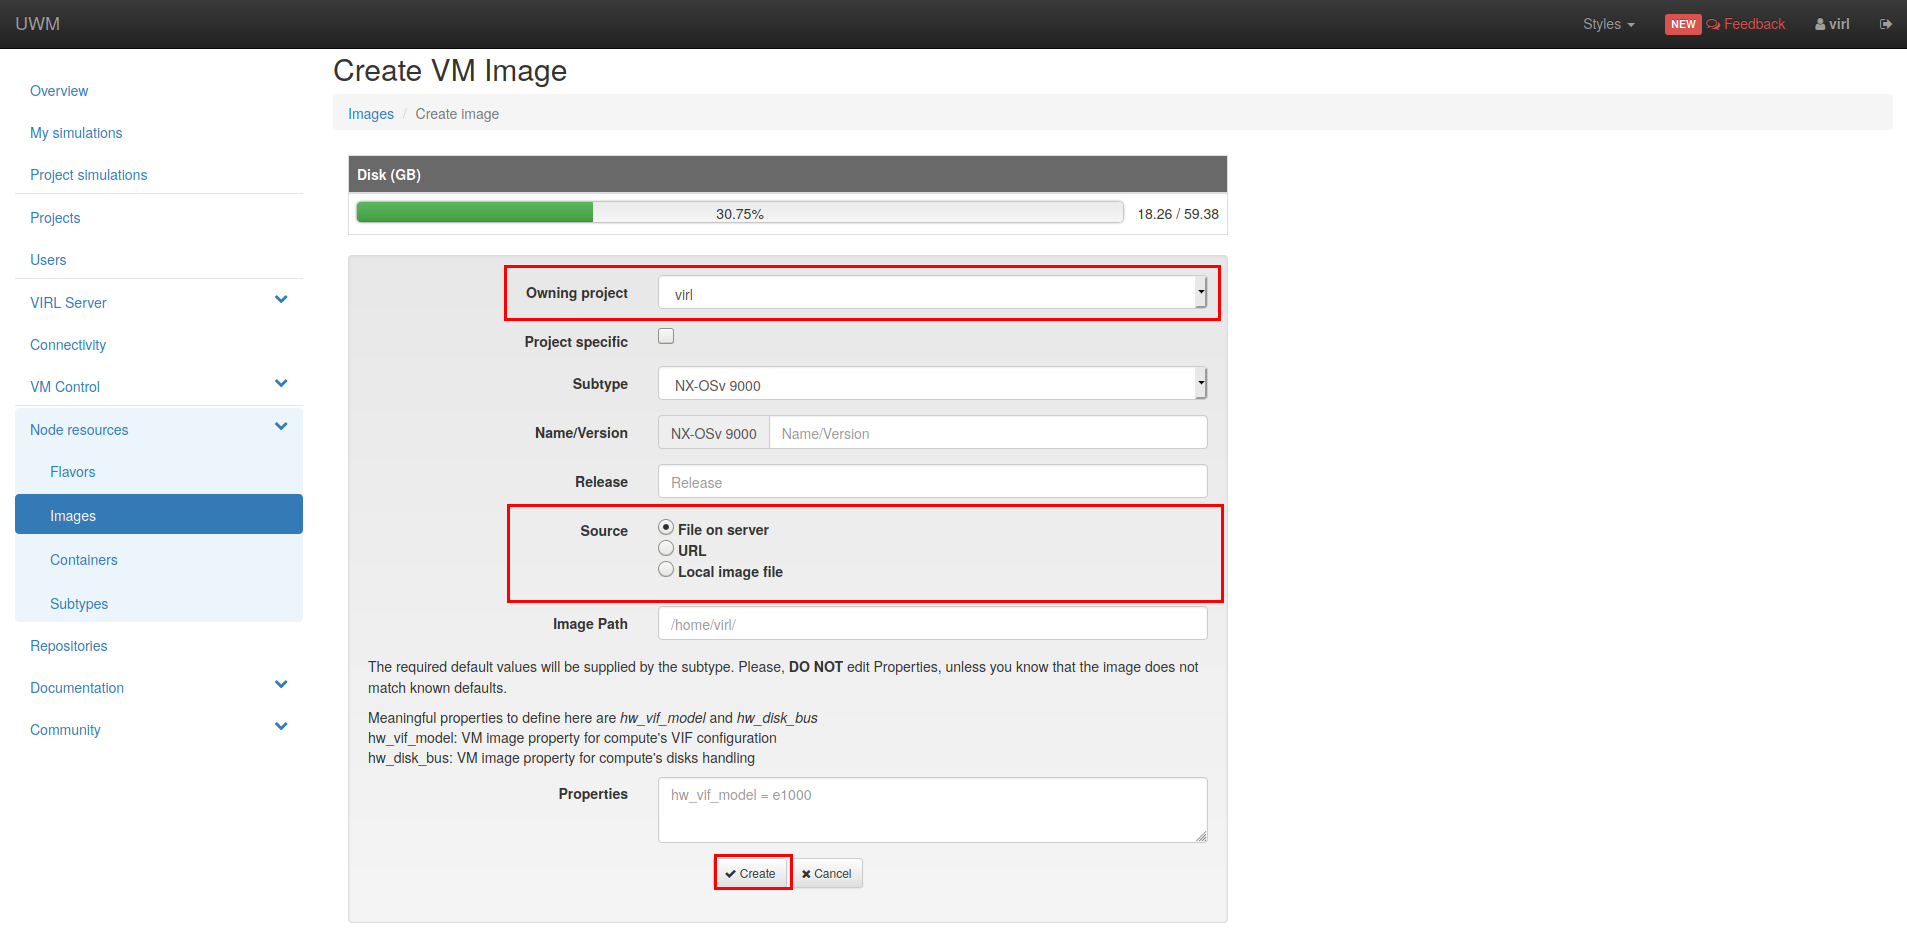
\includegraphics[width=\textwidth]{images/CreateVMimage.png}
\end{figure}

\begin{itemize}
	\item On top you can see how many space you still have on your disk.
	\item You can choose for what project and users you want to enable it.
	\item You have to select the correct Subtype and Source.
	\item And lastly you have to provide the image and create the VM image.
\end{itemize}

Now, to be able to use our new image, we have to make it available in the VIRL editor.
Ideally, this would happen automatically,
but since the VIRL editor is clearly still under heavy development,
we have to do it manually.
More specifically, you need to add the following code snippet to
\begin{verbatim}
/usr/local/lib/python2.7/dist-packages/autonetkit_cisco_webui/web_content/
sampleData/subtypes.json
\end{verbatim}

\begin{lstlisting}[caption=JSON code for NX-OSv 9000]
{
	"intfManagement": "mgmt0",
	"icon": "nx_osv",
	"intfNameFormat": "Ethernet1/{0}",
	"minIntfIndices": [
		1
	],
	"name": "NX-OSv 9000",
	"intfSegmentSizes": [
		0
	],
	"maxIntfIndices": [
		27
	],
	"visible": true,
	"serialConsoles": 2
}
\end{lstlisting}

\subsubsection{Interconnecting VIRL simulations and connecting to external networks}
In VIRL, it is possible to interconnect VIRL simulations
and to connect VIRL simulations to other external networks.
Interconnecting simulations is possible on both the DevNet sandbox platform and the VIRL PE,
connecting simulations to external networks is, for security reasons, only possible on the VIRL PE.

Interconnecting simulations is as easy as connecting adding a \textbf{FLAT} node
(found under the \textit{switches} group in the VIRL editor)
to each topology and ensuring they are connected both to the same link.

The \textbf{FLAT} node essentially connects the interface on your router
with a specifically defined bridge on your VIRL server.
So, connecting to an external network would seem as simple as adding a physical interface to the bridge.
The easiest way to do this correctly,
is in \textit{System Configuration} under the \textbf{VIRL Server} (1) tab in UWM
(login as \textbf{uwmadmin}).
Once there, navigate to \textit{Shared Networks} (2) $\rightarrow$ \textit{shared1 (flat)} (3)
and set the physical interface under \textit{Host Interface} (4).
You can change other settings too here, like your host ip-address, the ip-range for your virtual routers, \dots
When done, click \textit{Apply Changes} (5) and follow the on-screen instructions.
\begin{figure}[H]
	\centering
	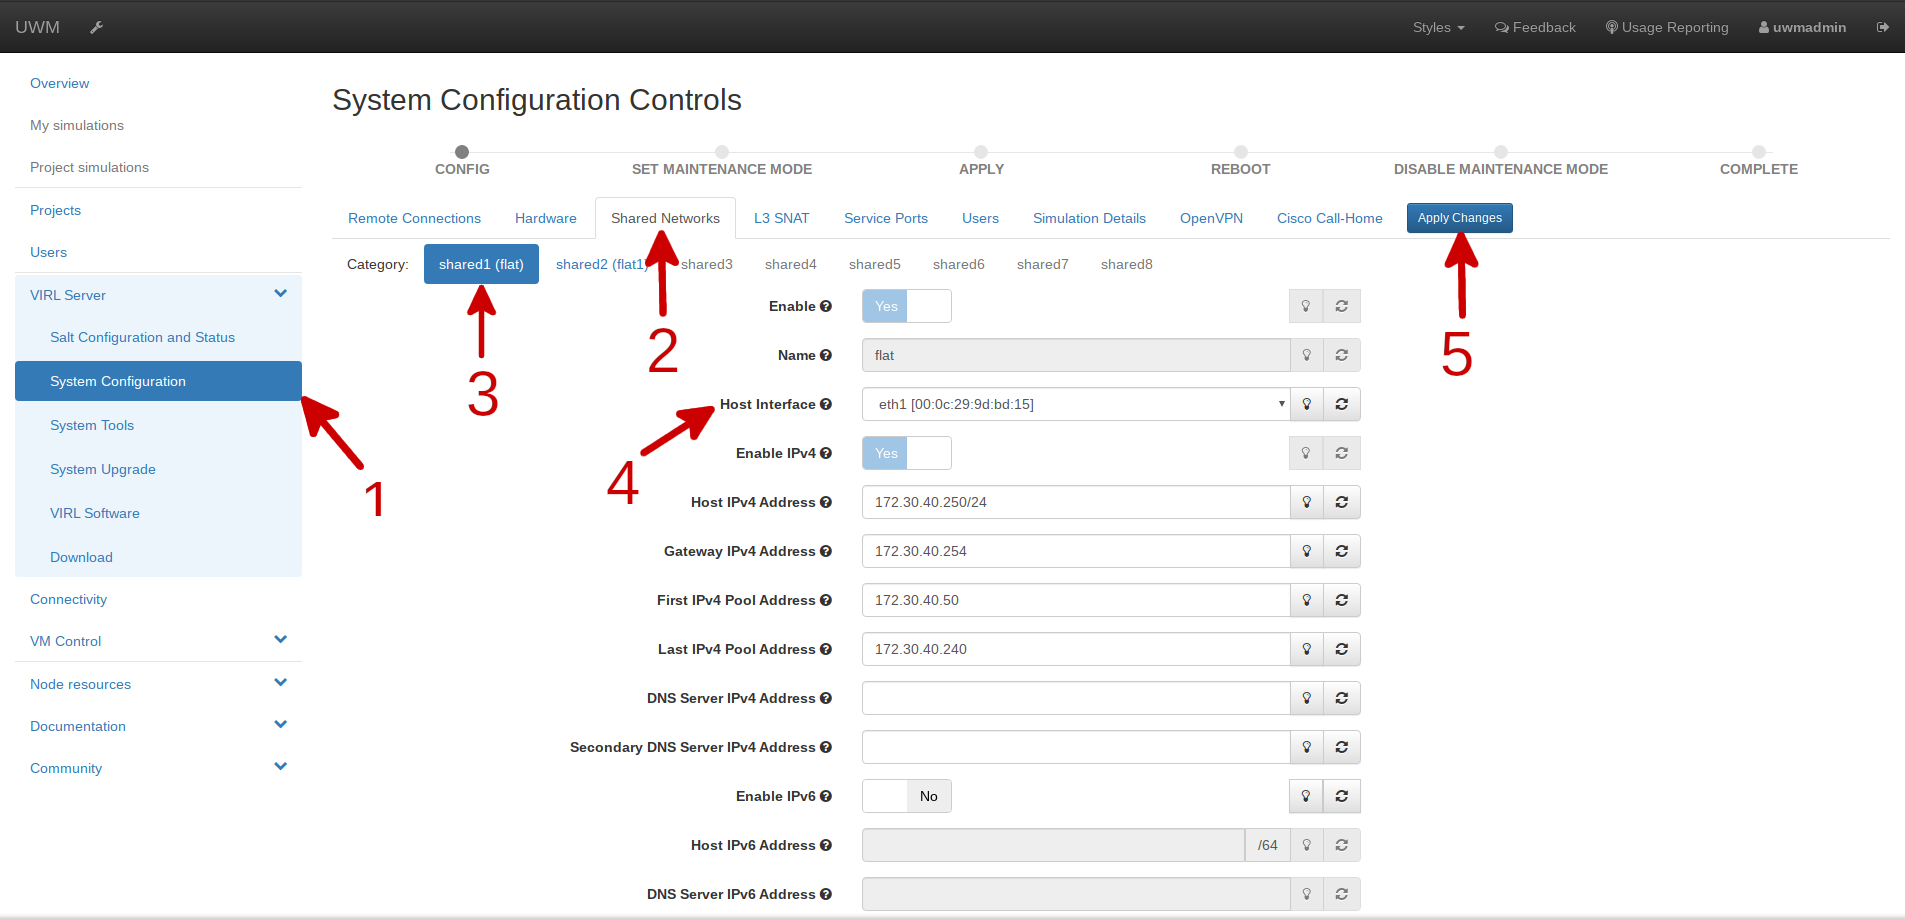
\includegraphics[width=\textwidth]{images/uwm_configure_flat.png}
	\caption{Configuring the \textit{flat} network}
\end{figure}

When running VIRL PE in an ESXi vm, you may need to enable \textit{promiscuous mode} for the used vSwitch.
\begin{figure}[H]
	\centering
	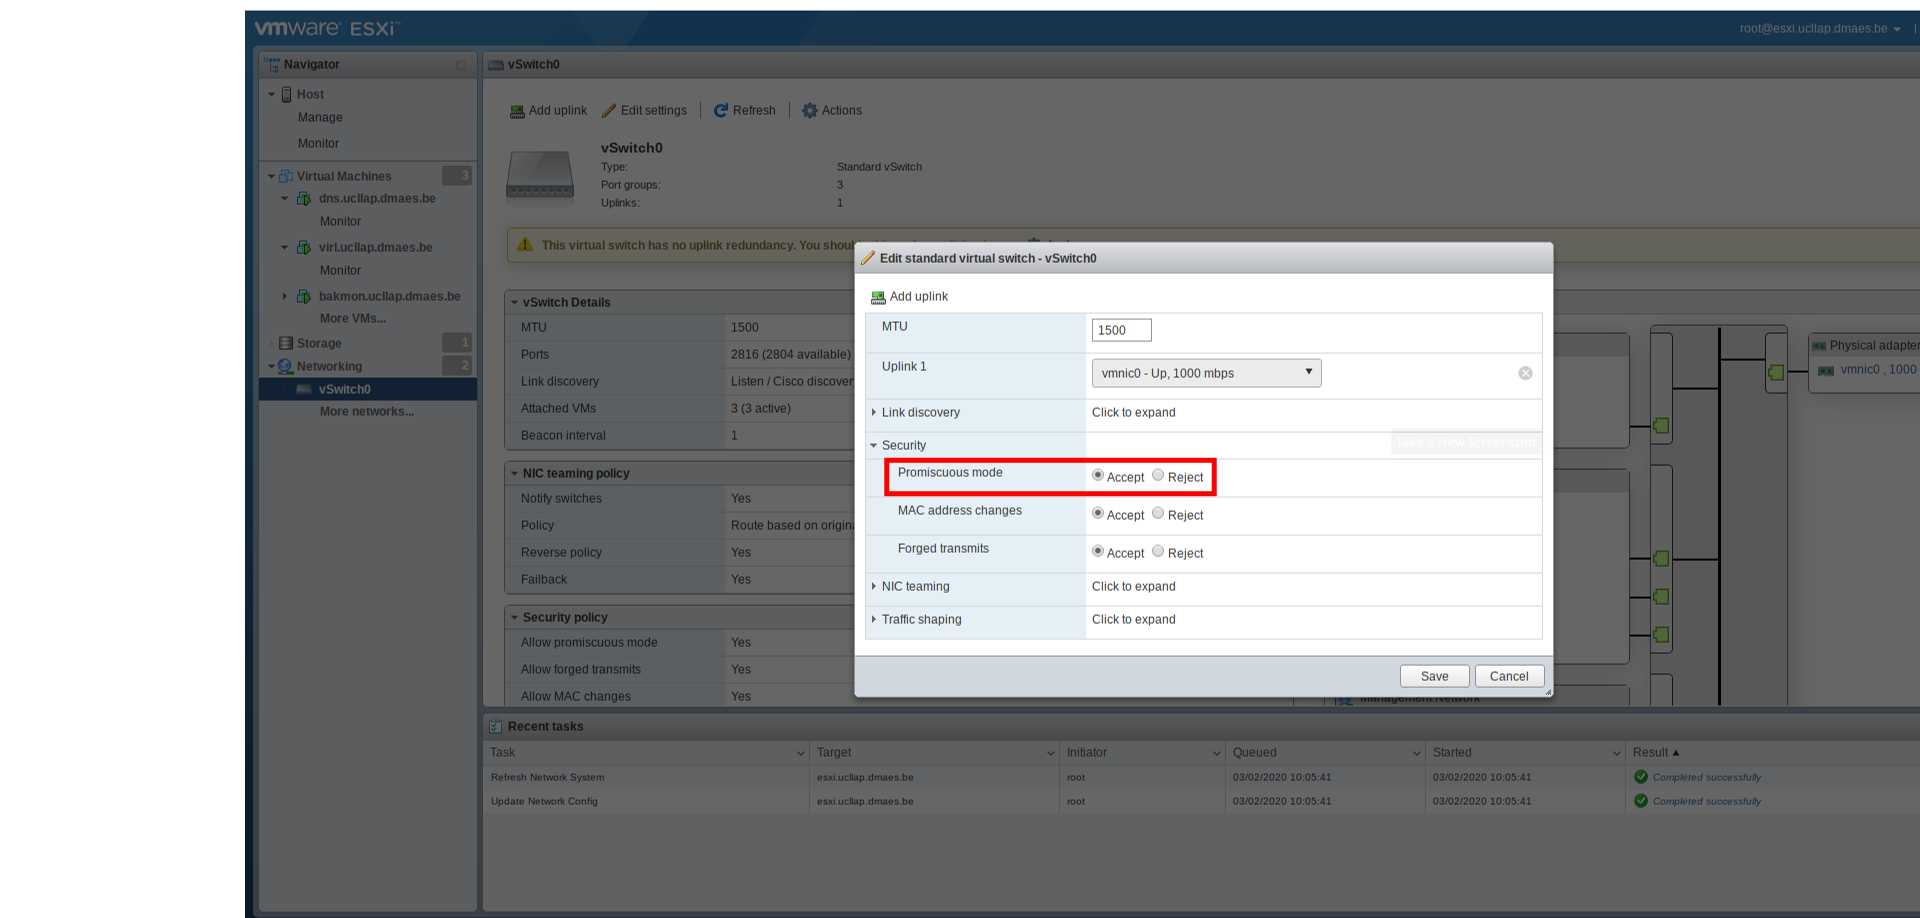
\includegraphics[width=\textwidth]{images/esxi_allow_promiscuous_mode.png}
	\caption{Enabling promiscuous mode in ESXi}
\end{figure}

\newpage
\section{Our test setup}
Using VIRL on your own hardware can be done quiet easily.
Downloading the ISO meant for bare-metal, installing it and
configuring users and interfaces, is enough to get started.

For practical reasons we made our setup a bit more complicated.
Firstly, this made work easier.
Secondly, we learned new stuff while building the setup,
and it could be used for another task given to us.

In detail, our setup exists of a gateway (we used VyOS) to manage networks
(the OpenVPN-network, used for external access, the private network, to which we connect when on-site,
the services network, which contains the VIRL server and DNS/backup server,
and the management network, used to manage gateway, switch and hypervisor),
a Cisco catalyst switch to connect devices to the those networks,
a ESXi-box to host our VMs, a DNS-VM, a VM for backup \& monitoring, 
and the VIRL-VM.

\subsection{Installation Guide}
I'll explain installing VIRL, LibreNMS and RANCID.
The other parts in our setup our just there for logistical reasons,
and will be different in any other setup.

\subsubsection{VIRL}
Installing VIRL is pretty simple and straightforward.
There are images provided for installation either on bare-metal or in ESXi.
We installed VIRL in ESXi, this allowed us to take snapshots of the machine on the one hand,
and use the same hardware for other services on the other hand.

Installation of VIRL in ESXi is done by downloading the provided .ova-file,
importing it in ESXi, and following the VIRL configuration prompt.
There isn't much more to it than setting users and passwords,
and assigning an interface for access to VIRL.

When all done, you can login to the VIRL-Web interface
and import your key as explained by the big yellow banner greeting you.

\subsubsection{LibreNMS}
Another question we got, aside from testing VIRL,
was to setup router/switch config-backups with RANCID in a change-based manner
instead of a time-based manner.

We did this by enabling SNMP-traps for configuration changes on our switch.
Then, we needed something that could catch those SNMP-traps and trigger a rancid-run.
Because LibreNMS is pretty easy to set up and comes with good support for SNMP-traps out-of-the-box, we chose this solution.

We suggest you follow the official documentation for setting up LibreNMS,
it is very straightforward: \url{https://docs.librenms.org/Installation/}

Sadly, LibreNMS does not have handlers for the right Cisco SNMP-traps
and only logs them.
However, writing your own handler is pretty easy and explained here:
\url{https://docs.librenms.org/Developing/SNMP-Traps/}

We wrote the following handler:

\begin{minipage}{\linewidth}
\begin{lstlisting}[caption=LibreNMS SnmptrapHandler for CISCO-CONFIG-MAN-MIB::ciscoConfigManEvent]
<?php
/** 
	* CiscoConfigChanged.php
	* 
	* Handles CISCO-CONFIG-MAN-MIB::ciscoConfigManEvent
*/

namespace LibreNMS\Snmptrap\Handlers;

use App\Models\Device;
use LibreNMS\Interfaces\SnmptrapHandler;
use LibreNMS\Snmptrap\Trap;
use Log;

class CiscoConfigChanged implements SnmptrapHandler {
	/**
		* Handle snmptrap.
		* Data is pre-parsed and delivered as a Trap.
		* 
		* @param Device $device
		* @param Trap $trap
		* @return void
		*/
	public function handle(Device $device, Trap $trap) {
		shell_exec('{{ librenms_ciscoConfigChanged }}');
	}
} 
\end{lstlisting}
\end{minipage}

Naturally, any other monitoring platform that can trigger arbitrary code on SNMP-traps can be used instead of LibreNMS.
The principle stays the same.

\subsubsection{RANCID}
RANCID is a platform for easy backups of networking devices.
Our setup is as default as it gets, and I suggest you follow this fine guide:
\url{http://www.linuxhomenetworking.com/wiki/index.php/Quick_HOWTO_:_Ch1_:_Network_Backups_With_Rancid}
We did, however, use Git instead of the default CVS for version-management.
Using git is as simple as setting \verb|RCSSYS=git;| in \verb|rancid.conf|,
before you run \verb|rancid-cvs|.


\newpage
\section{The UCLL core network}
\subsection{Current specific part of the core network that we virtualized}

\begin{figure}[H]
	\centering
	\includegraphics[width=\textwidth]{../diagrams/original_layer1.png}
	\caption{Layer one topology}
\end{figure}

\begin{figure}[H]
	\centering
	\includegraphics[width=\textwidth]{../diagrams/original_layer2.png}
	\caption{Layer two topology}
\end{figure}
\newpage
\subsection{Our implementation}
\subsubsection{The topology}

\begin{figure}[H]
	\centering
	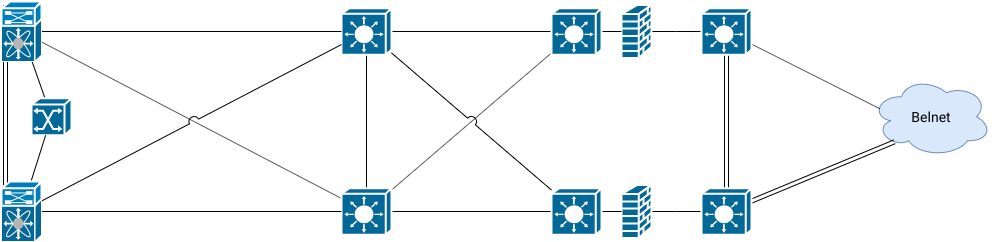
\includegraphics[width=\textwidth]{images/topology.png}
\end{figure}

For our project we altered the network based on the project requirements, the most important parts to focus on and limitations in VIRL.

That being said we will shortly discuss the alterations we made:
\begin{itemize}
	\item Mainly of course we didn't try to remake the whole core network all at once.
	We firstly focused on the up-link to Belnet, the Firewall, the core switches and the data center.
	\item With our limited part of the network we still had to figure out this implementation in VIRL.
	The machines didn't always do what we wanted them to do.
	For example the ASA machines weren't able to make Etherchannels so we had to put some extra switches between them and the core switches.
	\item Next we ran into some trouble withe the core switches being unable to do VSS.
	So we tried HSRP instead.
\end{itemize}

\newpage
\subsubsection{vPC}
On the 2 nexus switches in the topology, we configured vPC or Virtual Port Channel.
Port-channel is a technology that allows to aggregate multiple interfaces.
The traffic is then distributed between the connections.
vPC however provides a way to configure a port-channel across multiple switches, also known as vPC peers.
In our topology the 2 nexus switches appear as a single PortChannel to the layer3 switches.

\begin{figure}[H]
	\centering
	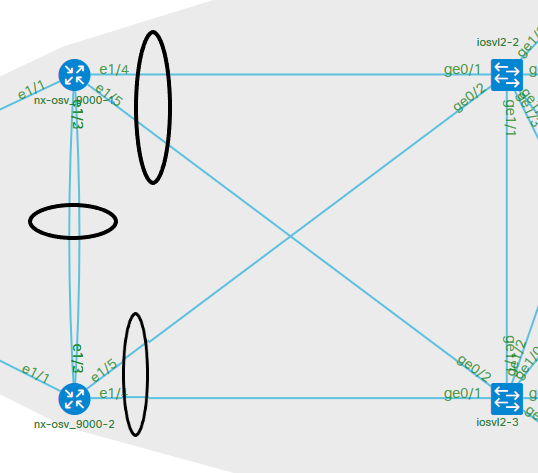
\includegraphics[width=\textwidth]{images/vPC.png}
\end{figure}

Part of the topology with the two nexus switches.

\begin{figure}[H]
	\centering
	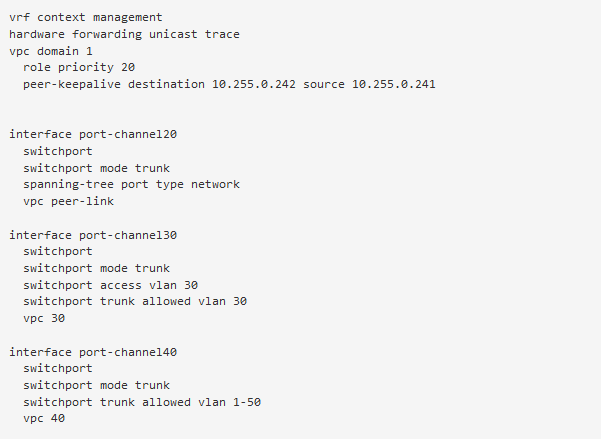
\includegraphics[width=\textwidth]{images/vPC_Config.png}
\end{figure}
Configuration file of one of the nexus 9k switches.

\newpage
\subsubsection{HSRP}
Instead of VSS we set up HSRP on the core switches.
We set up a virtual router toward \verb|asav-1| and another virtual router towards \verb|asav-2|.
Core switch 1 is for both virtual routers the active.

\begin{figure}[H]
	\centering
	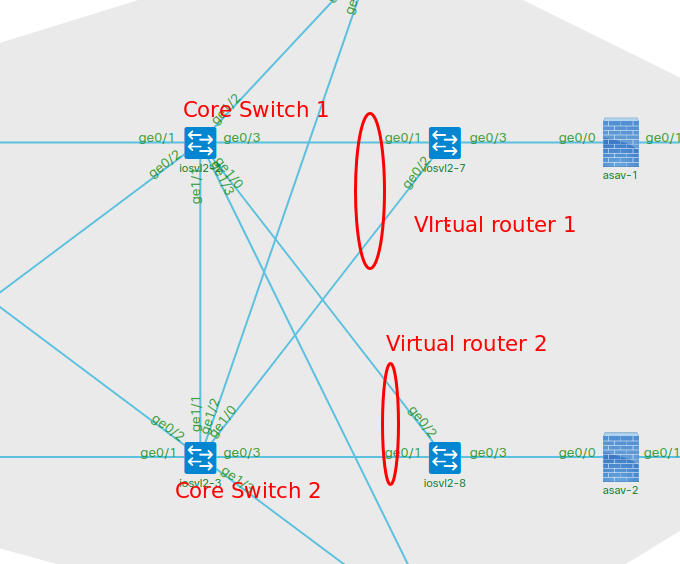
\includegraphics[width=\textwidth]{images/Hsrp.png}
\end{figure}

In the running-configuration you indeed see that the core switch 1 has the elevated priority and it will preempt when the priorities would switch.

\begin{figure}[H]
	\centering
	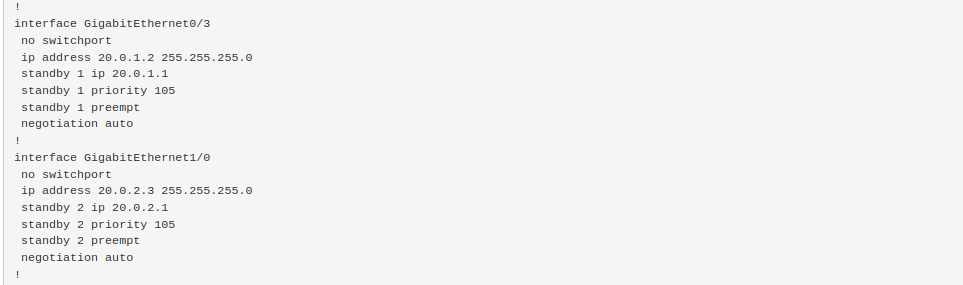
\includegraphics[width=\textwidth]{images/Hsrp_conf.png}
\end{figure}


\newpage
\subsubsection{BGP}

BGP or Border Gateway Protocol is a protocol to exchange routing information between autonomous systems (AS) on the internet.
In our topology we have two autonomous systems, Belnet and the UCLL. We gave Belnet the AS number two and the UCLL number one.
Between the 2 edge switches on the UCLL network we run iBGP. We also configured Etherchannel between the 2 edge switches and between Belnet and one of the switches.

\begin{figure}[H]
	\centering
	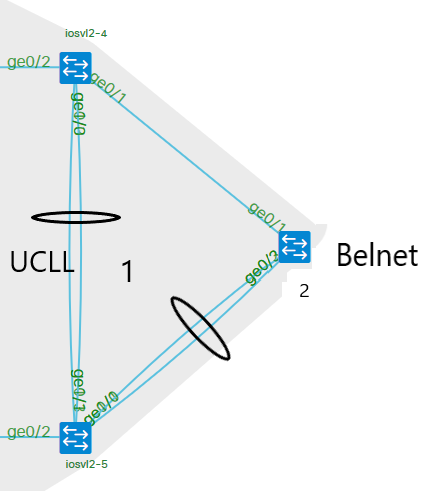
\includegraphics[width=\textwidth]{images/bgp_topologie.png}
\end{figure}

\newpage

\begin{figure}[H]
	\centering
	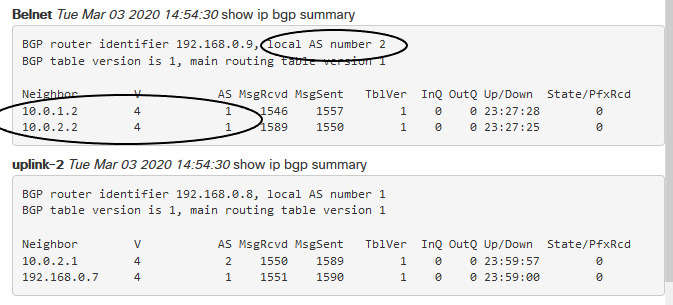
\includegraphics[width=\textwidth]{images/bgp_config.png}
\end{figure}

In these configuration file from the Belnet switch and one of the edge switches from the UCLL you can see their AS number, the neighbors, the AS number from the neighbors \dots
\newpage
\subsubsection{The ASA cluster}

We encountered some trouble trying to configure the ASA machines on VIRL to form an ASA cluster. Firstly there was a lot of confusing information on the internet. Next we encountered trouble with the ASA machines not being able to form Etherchannels. So we added extra switches between the HSRP switches and the cluster.

After consultation it appeared better to try and configure the ASA cluster with the ASDM GUI.So pretty late in the project we researched a little topology to connect to the GUI but we lacked the resources to run it on our machine next to our main topology and it was not possible to do on the Devnet solution. So sadly we had to leave this configuration unconquered. It should be possible to configure them except for the fact that they can't configure Etherchannels.

\newpage
\subsubsection{Vrf lite}
Since the core network runs multi area OSPF per Vrf we also tried to implement some vrf's. With a vrf you are splitting up a router into multiple virtual routers. But since vrf works on layer 3 and vlans on layer 2 it gave us some trouble at the end of our project. We decided to not focus our time in solving this problem since we had already succeeded in setting up Vrf all by it self.

In the next images you will see the vrf set up in another topology. In this topology we made 2 Vrf's on the iosv-1 router. One towards iosv-2 called UP and one towards iosv-3 called DOWN. The Mgmt-intf vrf is set by the ANK.


\begin{figure}[H]
	\centering
	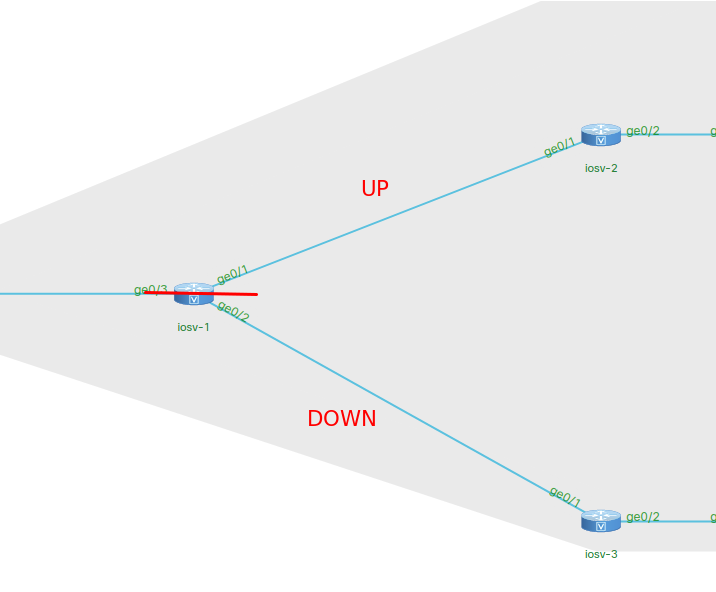
\includegraphics[width=\textwidth]{images/Vrf.png}
\end{figure}

\begin{figure}[H]
	\centering
	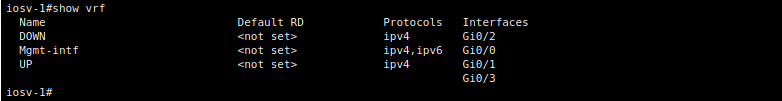
\includegraphics[width=\textwidth]{images/Vrf_show.png}
\end{figure}


\newpage
\subsubsection{BFD}
BFD or Bidirectional forwarding detection is a detection protocol to provide a fast way to detect a path failure. BFD can also be used for network administrators because it detects failures at a uniform rate.
We used BFD on the Layer three switch from Belnet and on one of the L3 edge switches from the UCLL where we also configured BGP and OSPF.

\begin{figure}[H]
	\centering
	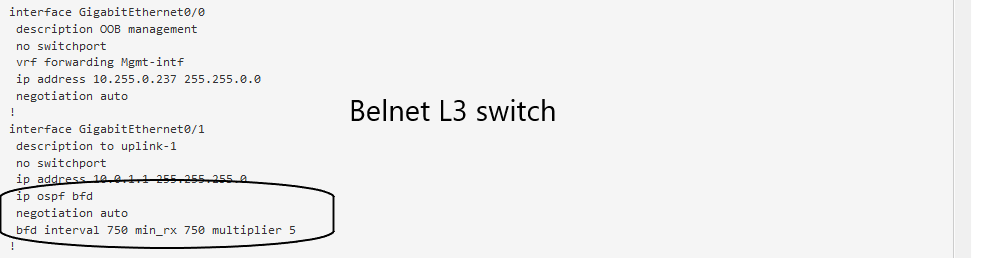
\includegraphics[width=\textwidth]{images/Bfd.png}
\end{figure}

\newpage

\section{Links}
\begin{description}
	\item [Cisco configuration pages] \url{https://www.cisco.com/}
	\item[Cisco DevNet] \url{https://devnetsandbox.cisco.com}
	\item[Cisco LearningNetwork] \url{https://learningnetwork.cisco.com}
	\item[VIRL setup documentation] \url{http://get.virl.info/index.php}
	\item[ESXi] \url{https://my.vmware.com/en/web/vmware/evalcenter?p=free-esxi6}
	\item[VyOS] \url{https://www.vyos.io/}
	\item[RANCID] \url{https://www.shrubbery.net/rancid/}
	\item[LibreNMS] \url{https://www.librenms.org/}
\end{description} 

\end{document}
